\section{Autonomous landing algorithm}
\label{sec:algo}

 This section describes the conditions that need to be satisfied in order to achieve safe landing. These are 
 illustrated using high resolution bathymetric data collected by the vehicle BOSS-A at the Takuyo Daigo seamount during the KR$16$-$01$ cruise of R/V Keirei \cite{Thornton2013l,Nishida2016}. The specifications of the laser mapping system used to collect the data are given in Table~\ref{t:table1}. These landing conditions are used to develop an autonomous landing algorithm that consists of the following steps:

\begin{itemize}
  \item \textit{Surface mapping:} Convert high resolution point clouds generated by the mapping system into a bathymetry surface with uniform lateral resolution.
  \item \textit{Landing area detection:} Identify landing areas within sections of bathymetry that satisfy the criteria for safe landing developed in this work.
  \item \textit{Site identification:} Within the detected landing areas, identify candidate landing sites that are large enough for a vehicle of defined geometry to fit along a certain heading. 
  \item \textit{Site selection:} Landing site properties are extracted for all the candidate sites and a cost function is defined to assess their suitability. The site with minimum landing cost is selected for landing site.
\end{itemize}


\begin{table}[!ht]
\centering
\caption{Properties of the mapping system}
\begin{tabular}{  |p{6cm}  p{4cm}| }
\hline
\textbf{Property} & \textbf{Value}\\ \hline 
Mapping altitude $a$ & $2$ m \\
Baseline between camera and laser $b$ & $1.03$ m\\
Vertical mounting angle of camera $\phi_m$ & $70^\circ$ \\
Horizontal opening angle of camera $\phi_h$ & $60.2^{\circ}$\\
Vertical opening angle of camera $\phi_v$ & $50.4^{\circ}$\\
Along-track resolution & $4$ mm\\
Cross-track resolution & $3$ mm\\
Vertical resolution & $6$ mm\\
\hline
\end{tabular}
\label{t:table1}
\end{table}

\subsection{Surface mapping}
\label{sub:mapping}

 Fig.~\ref{sf:mehul4a} shows a $25$\,m section of laser bathymetry mapped at a heading of $230^\circ$ using the method described by Bodenmann et al.,  \cite{Bodenmann2016}. Each point in the point cloud 
has a known position in the north, east and depth directions. The unstructured points are resampled to a uniform lateral grid resolution of $g_{res}=10$\,mm, as shown in (see Fig.~\ref{sf:mehul4b}). This resolution is chosen as it is sufficiently high to resolve any surface protrusions that may affect landing.

\begin{figure}[!ht]
\centering
\subfloat[Top view ortho projection of a 3d seafloor color reconstruction (left) and its corresponding hill shaded depth map (right).\label{sf:mehul4a}]{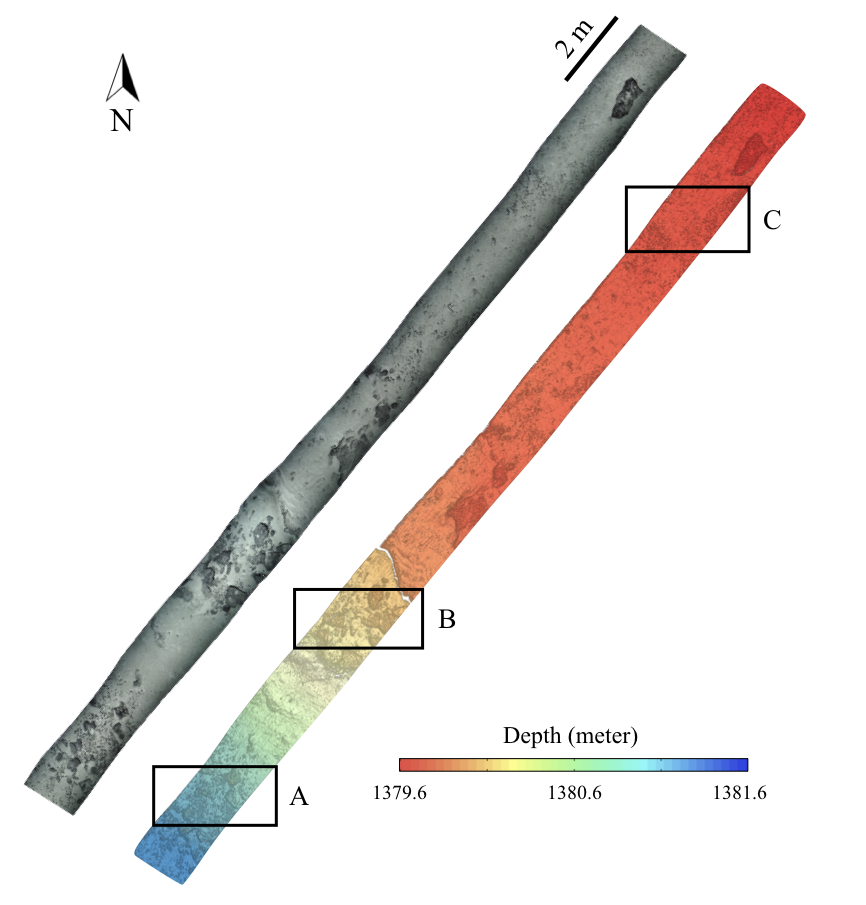
\includegraphics[width=5in]{./images/mehul4a.png}}\quad
\subfloat[Detailed views of bathymetric data resampled to a uniform lateral grid resolution of $g_{res}=10$\,mm, corresponding to the three areas A,B and C in Fig.~\ref{sf:mehul4a}.\label{sf:mehul4b}]{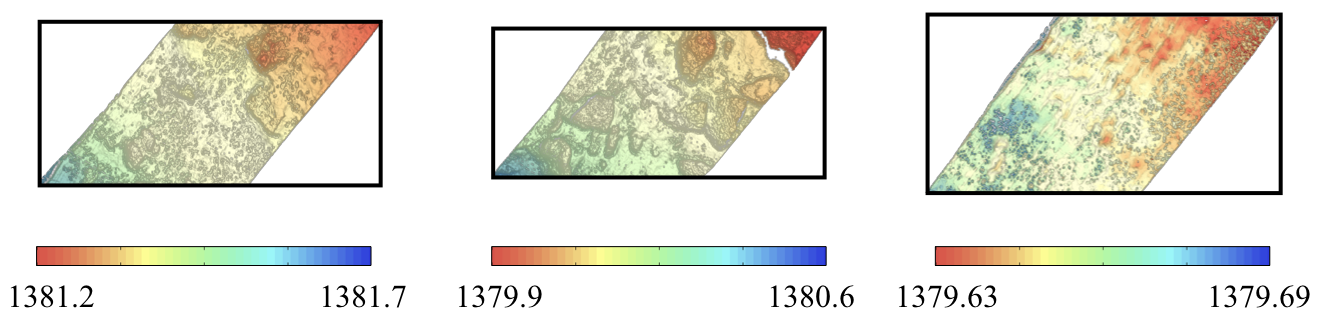
\includegraphics[width=7in]{./images/mehul4b.png}}
\caption{Seafloor bathymetry mapped using the high resolution laser mapping system mounted on the vehicle\label{sf:mehul4}}
\end{figure}


\subsection{Landing area detection}
\label{sub:landingarea}

In order to detect safe landing areas, a number of physical conditions need to be locally satisfied in the bathymetry. The effects of slope on landing are analyzed considering the vehicle's righting moment, seafloor friction and currents. The effects of protrusions on landing are analyzed considering their height. The vehicle parameters needed to judge safe landing are illustrated in Fig.~\ref{f:mehul5}, with specific values used in this study shown in Table~\ref{t:table2}. 
 
\begin{table}[!ht]
\centering
\caption{Physical properties of underwater platform}
\begin{tabular}{ | p{4cm}  p{6cm} p{4cm} | }
\hline
\textbf{Property} & \textbf{Description} & \textbf{Value}\\ \hline 
$l_u$ & length of landing vehicle & $1.7$ m\\
$b_u$ & width of landing vehicle & $0.5$ m\\
$h_u$ & height of landing vehicle & $0.45$ m\\
$F_G$ & force of  gravity (for $65$ Kg mass) & $637$ N \\
$F_B$ & force of buoyancy (for $62$ Kg mass) & $608$ N \\
$F_R$ & net  downward force  & $29$ N \\
$d_g$ & vertical distance to $C_G$ & $0.25$ m \\
$d_m$ & vertical distance between $C_G$ and $C_B$ & $0.05$ m \\
\hline
\end{tabular}
\label{t:table2}
\end{table}

\begin{figure}[!ht]
\centering
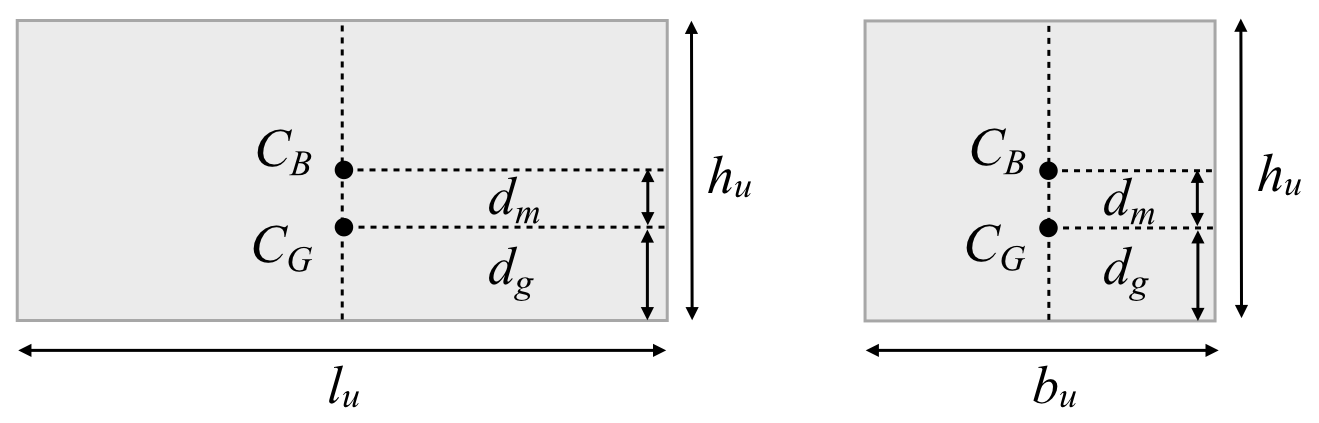
\includegraphics[width=5.0in]{./images/mehul5.png}
\caption{Side and top view of an vehicle with parameters used to determine landing conditions}
\label{f:mehul5}
\end{figure}

\subsubsection{Sloping surfaces}

The criteria for landing success is considered as when the vehicle can remain stationary and in full contact with the seafloor. Here, we determine the minimum slope on which an vehicle of known geometry and righting moment can meet this condition. The analysis is performed along different vehicle orientations, $\psi$, to find the maximum slope  $\theta_c$ where successful landing is possible (see Fig~\ref{f:mehul6}). 

While landing, the vehicle first makes contact with the slope along its smaller edge $b_u$ for orientations $0^\circ$ and $90^\circ$ and longer edge $l_u$ for orientations $180^\circ$ and $270^\circ$. For all other orientations, the vehicle makes contact on one of its corners.

\begin{figure}[!ht]
\centering
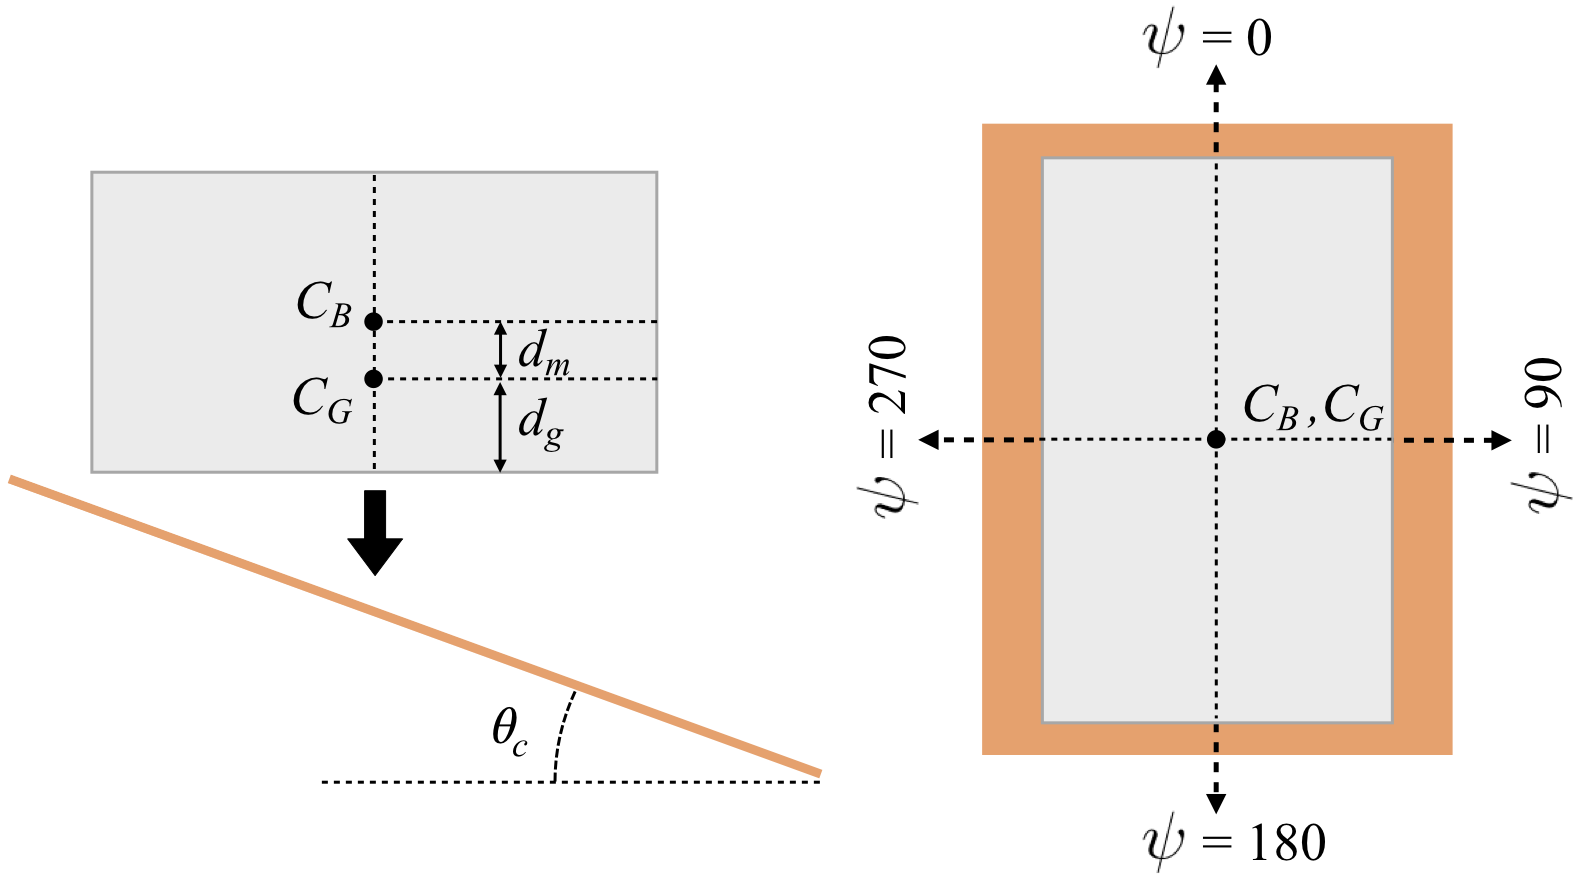
\includegraphics[width=5in]{./images/mehul6.png}
\caption{Side and top view of an vehicle landing on a slope}
\label{f:mehul6}
\end{figure}

\begin{figure}[!ht]
\centering
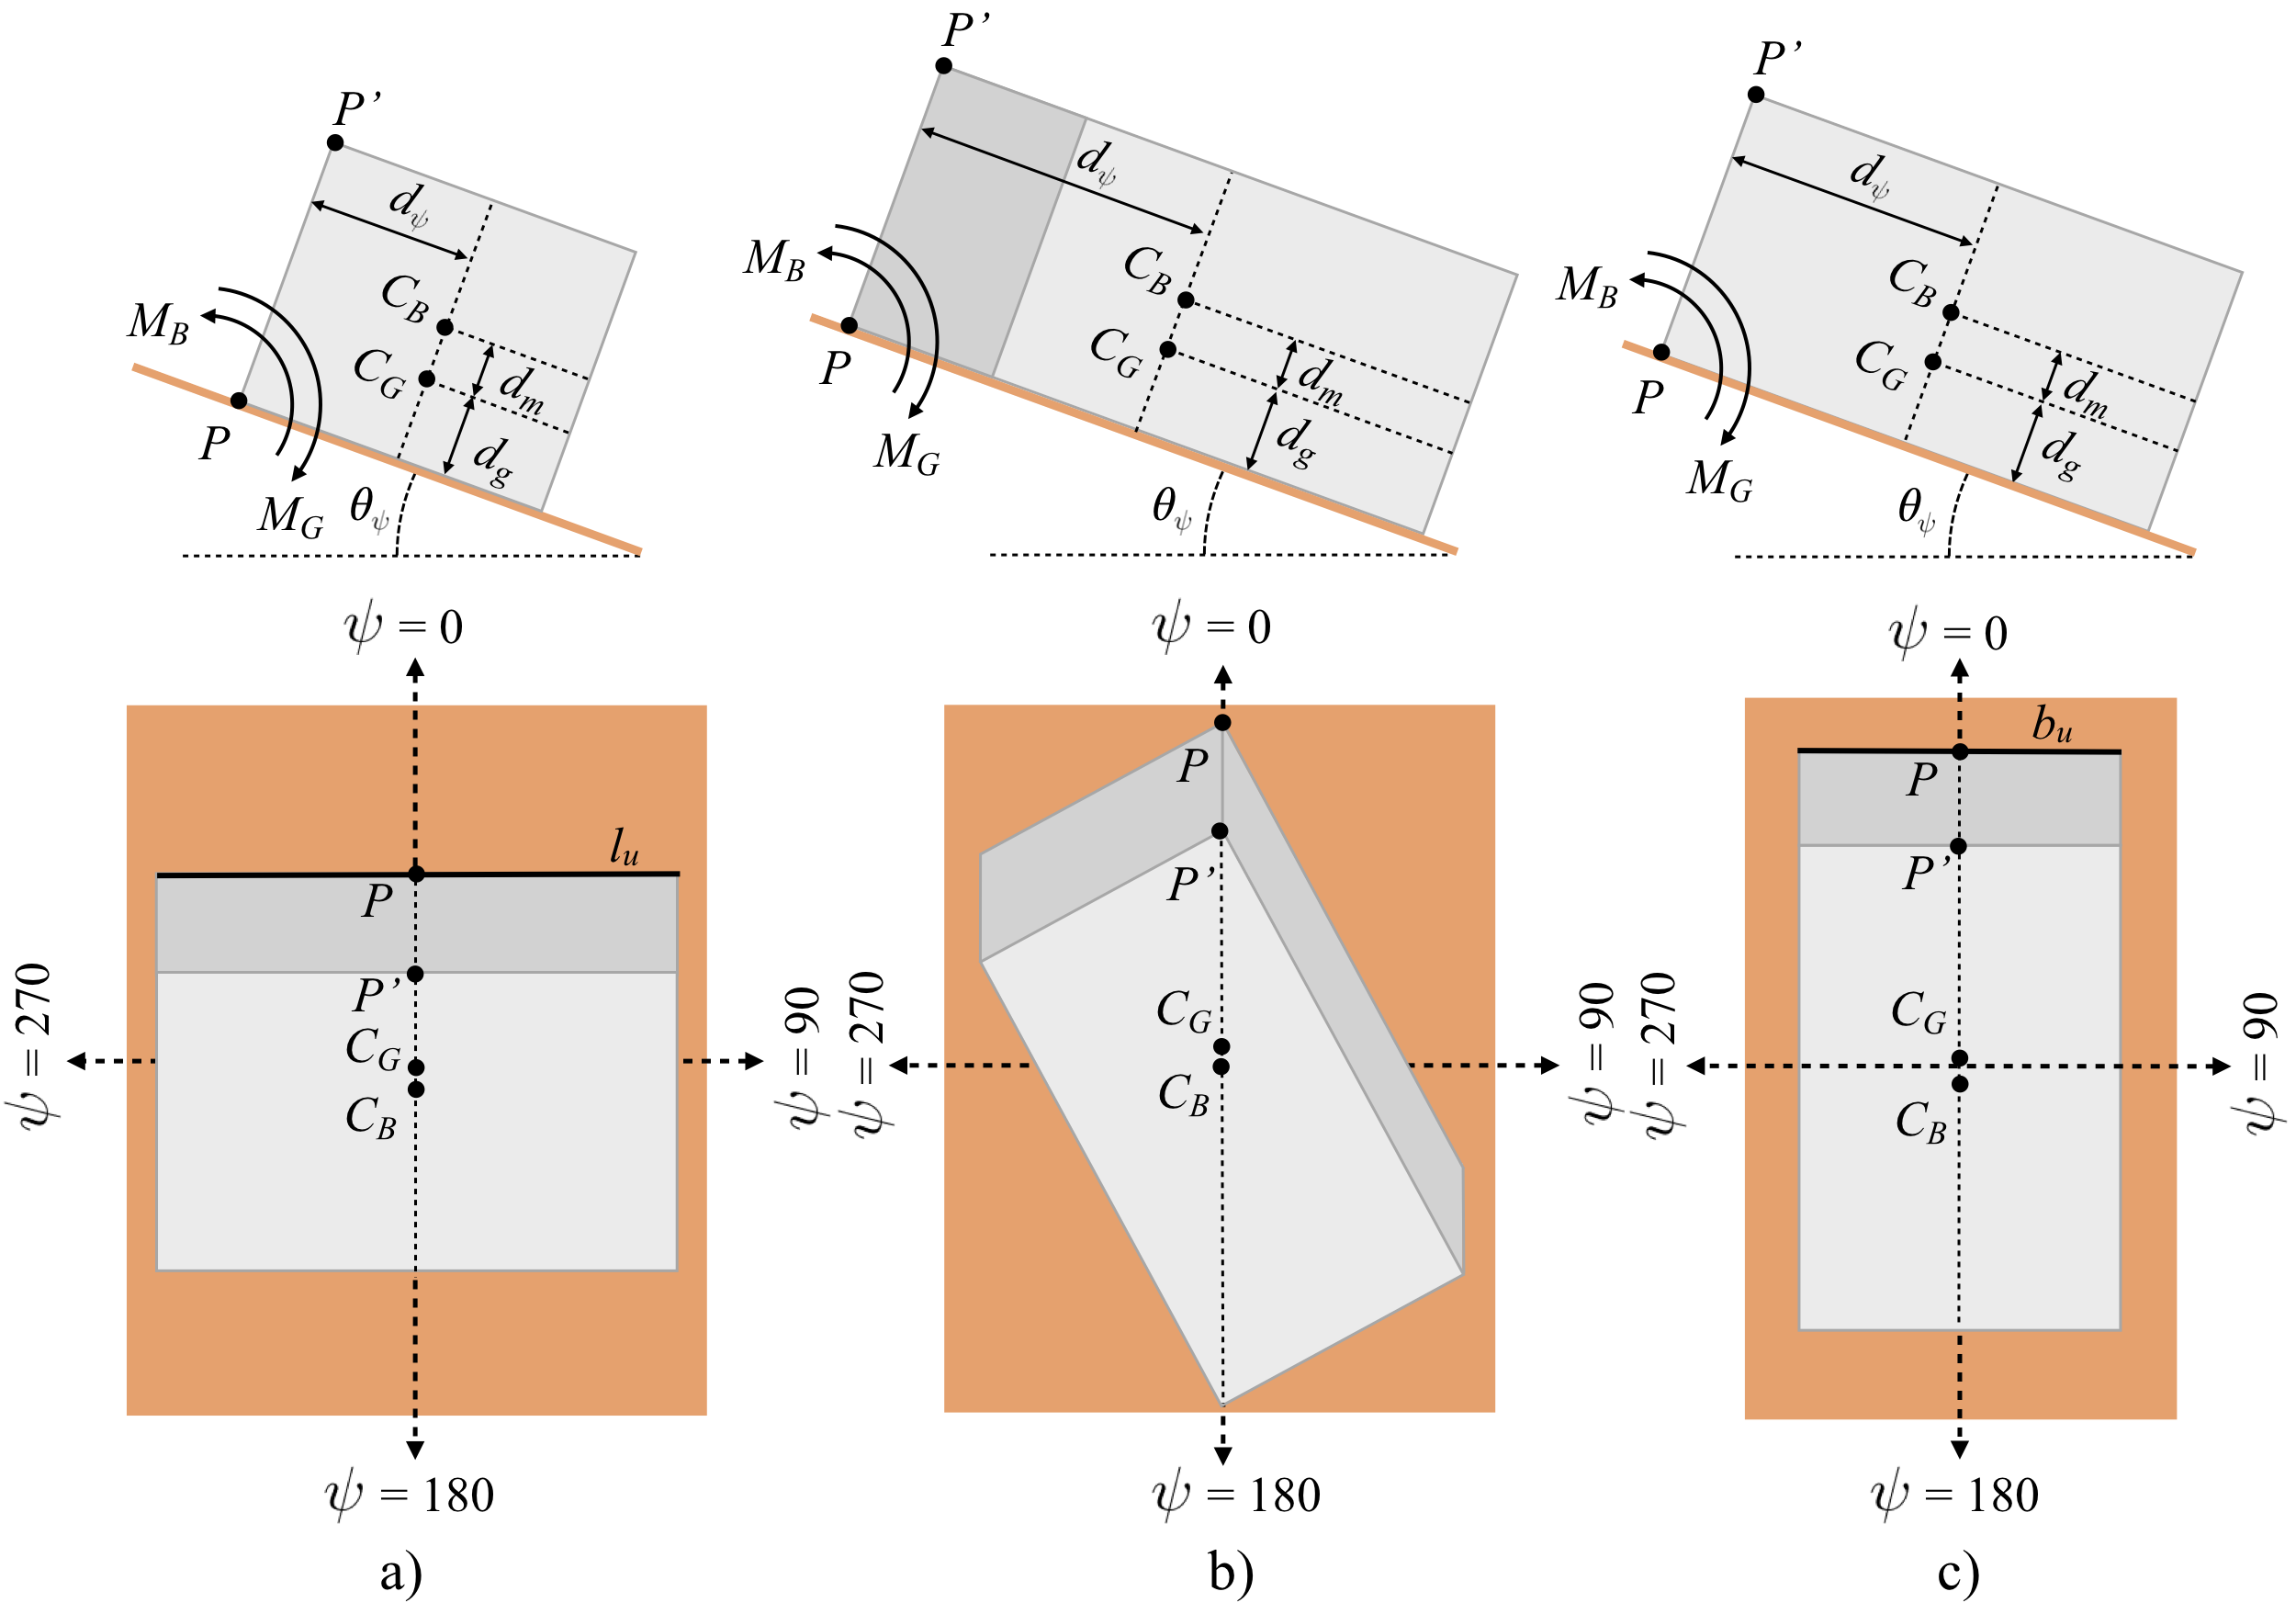
\includegraphics[width=7in]{./images/mehul7.png}
\caption{vehicle landing on a slope along different orientations}
\label{f:mehul7}
\end{figure}

To land successfully, the vehicle should settle flush with the slope of the seafloor. Once part of the vehicle makes contact with a sloped seafloor, the vehicle rotates along the plane formed by $C_G$, $C_B$, point $P$ and $P$' as shown in Fig~\ref{f:mehul7}. Since the vehicle's maximum tilt angle is determined by the vehicle's righting moment, the maximum angle of rotation is given by the equation
\begin{equation}
\label{eq:eq1}
\centering
	\theta_\psi = \tan^{-1}\left[ \frac{(d_{\psi} \times F_R)}{(d_m \times F_B) - (d_g \times F_R)}\right],
\end{equation}

\noindent where the distance $d_{\psi}$ is determined by the orientation of the vehicle, $\psi$, with respect to the slope. When landing along an edge, or along a diagonal axis as seen in Fig~\ref{f:mehul7}, the vehicle can make full contact with the surface while tilting along a single axis. For all other orientations, the vehicle rotates along a single axis until one of its edges makes contact with the slope after which it rotates about that edge to make full contact with the surface. 


Fig~\ref{f:mehul8} shows the maximum slope $\theta_c$ where the landing criteria can be met for along relative  vehicle orientations $\psi$ from $0^\circ$ to  $360^\circ$. Simulations are performed for vehicle aspect ratios ($l_u/b_u$) of $1$, $2$ and $4$ respectively. Since the minimum value of $\theta_c$ occurs when then vehicle lands on its shorter edge $l_u$, the maximum slope $\theta_c$ on which the vehicle can land can be determined by letting $d_{\psi} = 0.5 \times b_u$ in Equation~\ref{eq:eq1}, giving

\begin{equation}
\label{eq:eq2}
\centering
	\theta_c = \tan^{-1}\left[ \frac{(0.5 \times b_u \times F_R)}{(d_m \times F_B) - (d_g \times F_R)}\right].
\end{equation}

\begin{figure}[!ht]
\centering
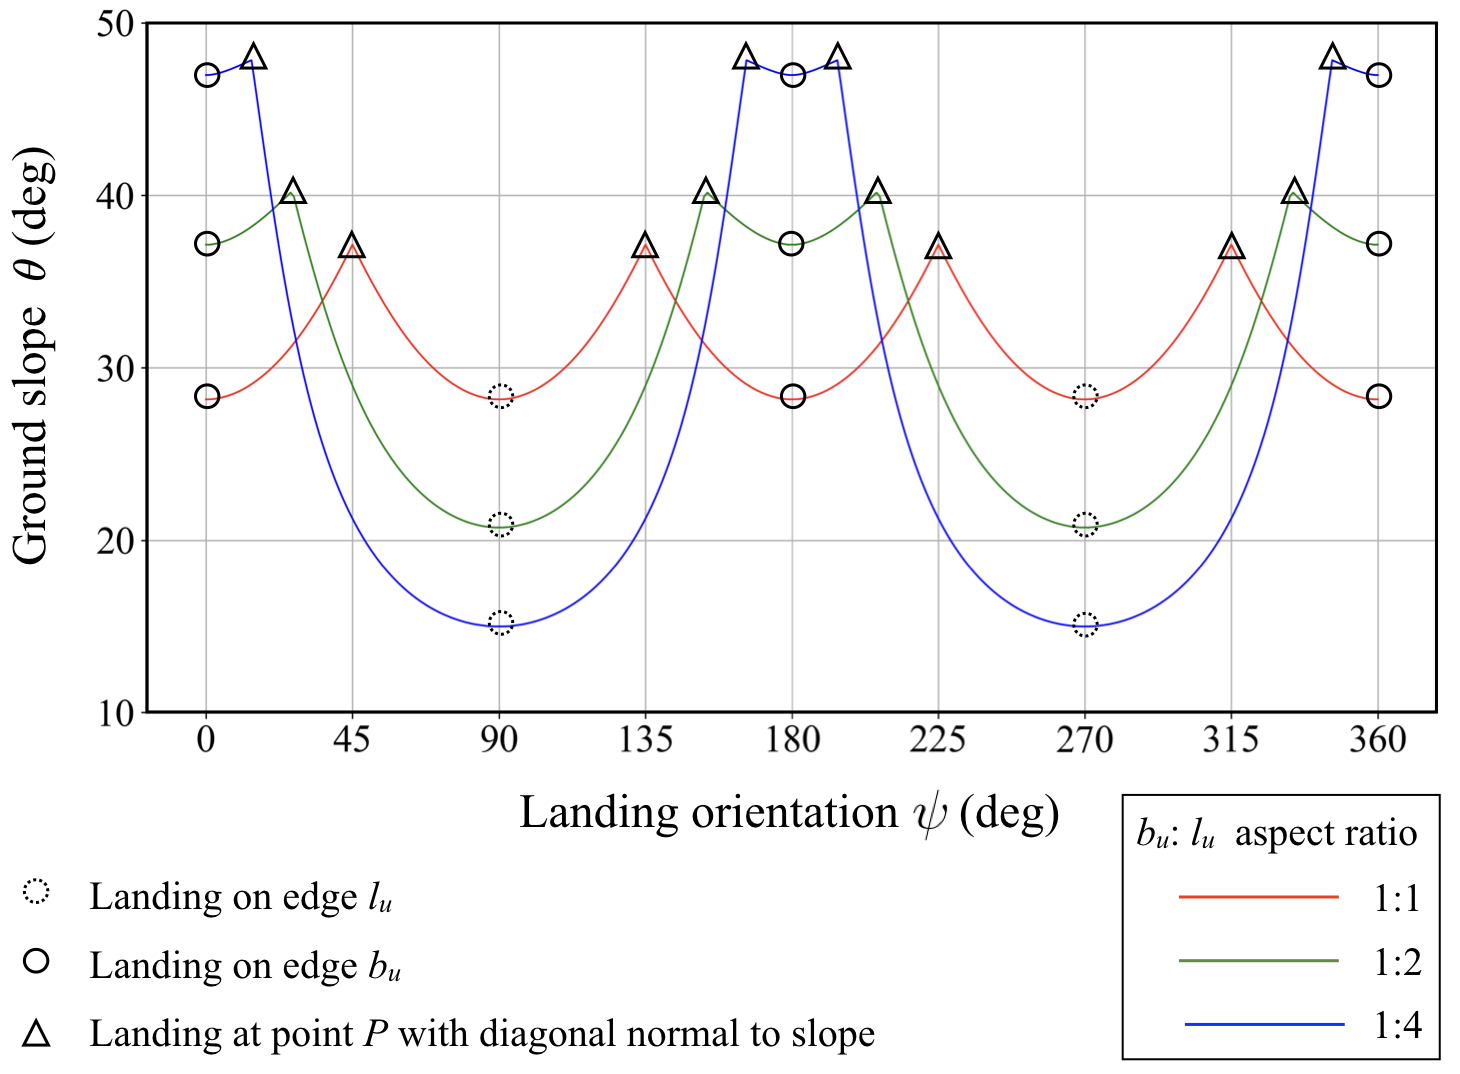
\includegraphics[width=6in]{./images/mehul8.png}
\caption{Maximum landing slope $\theta_c$ calculated for different landing orientations and aspect ratios of the vehicle}
\label{f:mehul8}
\end{figure}

\noindent For the vehicle parameters in Table.\ref{t:table2}, this gives a maximum slope on which the vehicle can land at any orientation of $\theta_c=17.7^\circ$.

For the vehicle to remain stationary on a slope once it has landed, the frictional force $F_F$ needs to be greater than or equal to the sum of the component of gravity $F_G$ acting along the slope in the downwards direction and the force due to seafloor currents $F_C$ pushing the vehicle down the slope. Fig~\ref{f:mehul9} illustrates this worst case scenario, where for the purpose of the simulation we neglect the effects of hydrodynamic lift. The steepness of the slope that the vehicle can remain stationary on depends on the frictional coefficient $\mu$ between the vehicle and seafloor. The relationship between the velocity of seafloor currents $v$ and the maximum slope on which the vehicle does not slip with its longer edge $l_u$ across the slope is calculated for a drag coefficient $C_d = 1.02$ and density $\rho= 1025$ Kg/m$^3$, the velocity of seafloor currents is then calculated as:
\begin{equation}
\label{eq:eq3}
\centering
	Fc = (F_G - F_B) \times (\mu \cos\theta - \sin\theta)
\end{equation}

\begin{equation}
\label{eq:eq4}
\centering
	v_c = \sqrt{ \frac{2 \times Fc}{C_d  \times  \rho  \times  l_u \times h_u}}
\end{equation}

\begin{figure}[!ht]
\centering
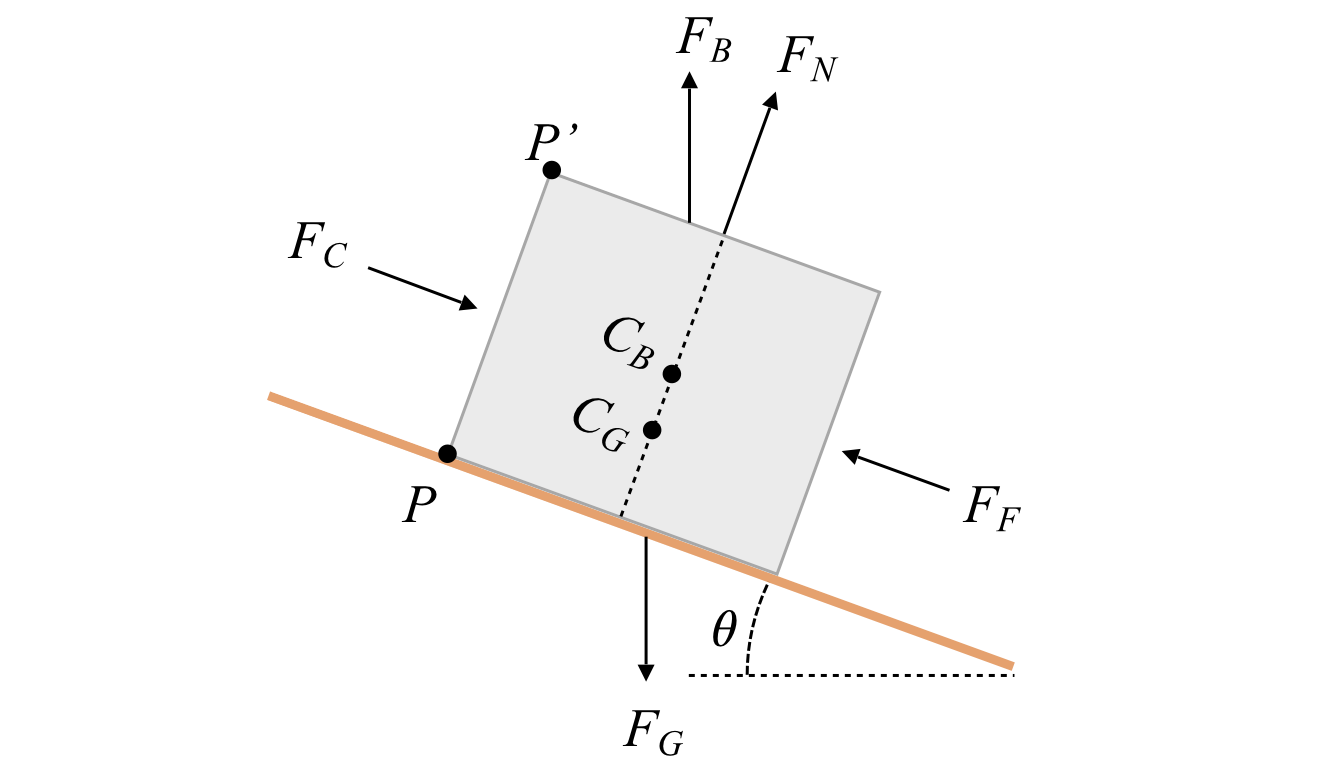
\includegraphics[width=6in]{./images/mehul9.png}
\caption{Forces acting on the vehicle after landing on the sloping surface}
\label{f:mehul9}
\end{figure}

\noindent The frictional coefficient of the seafloor typically varies between $0.1$ and $0.6$~\cite{DNV2017} with seafloor currents in the deep ocean typically $<0.2$\,m/s 
~\cite{Hollister1972}. The effects of friction and current on landing is calculated for slopes of between $0^\circ$ and $35^\circ$. The slope values calculated can be seen in Fig.~\ref{f:mehul10} where the area under each curve represents the conditions where the vehicle remains stationary. For a slope of $\theta_c = 17.7^\circ$ determined for the vehicle in Table.\ref{t:table2}, it can be seen that the vehicle will remain stable for currents under $0.14$ m/s and coefficient of friction more than $0.32$, which is reasonable for most deep-sea application.

\begin{figure}[!ht]
\centering
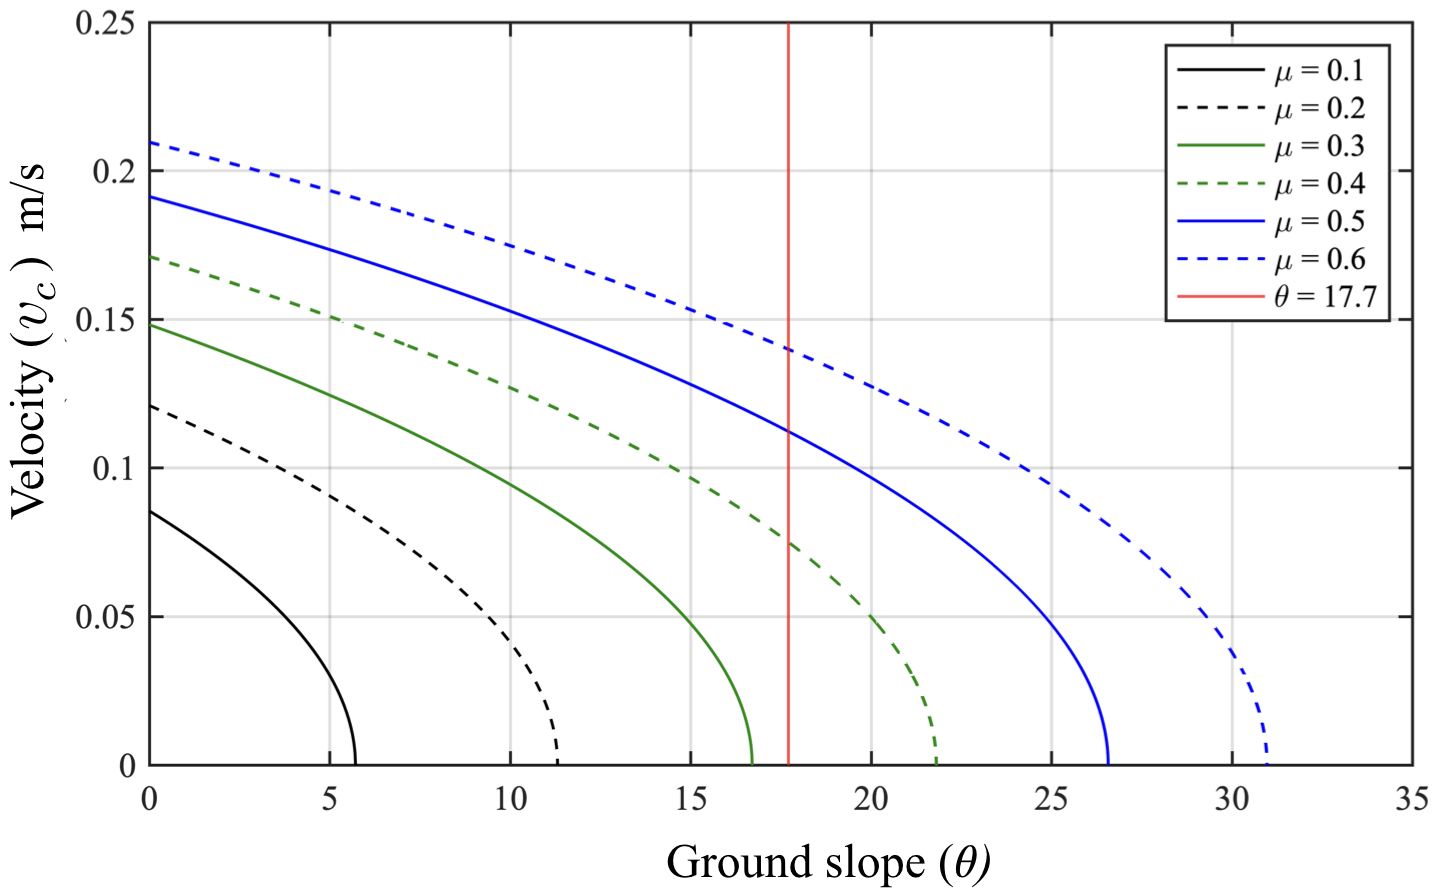
\includegraphics[width=4.5in]{./images/mehul10.png}
\caption{Analysis of seafloor currents and friction on the ground slope}
\label{f:mehul10}
\end{figure}

\subsubsection{Seafloor protrusions}

\begin{figure}[!t]
\centering
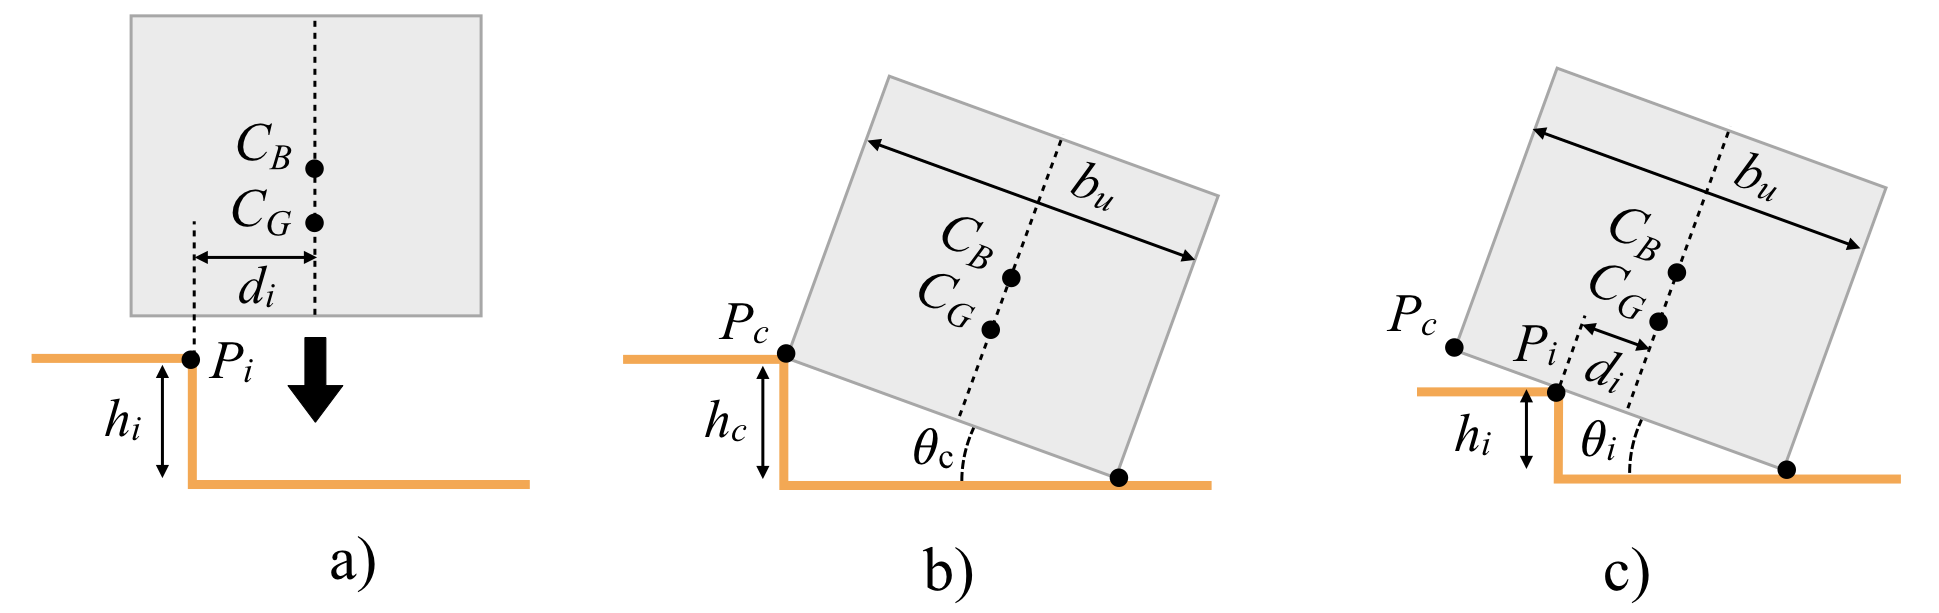
\includegraphics[width=\textwidth]{./images/mehul11.png}
\caption{a) Vehicle landing on an object on the seafloor b) Extreme condition of landing on an object c) Landing at a point between extreme condition and the centre line}
\label{f:mehul11}
\end{figure}

Seafloor rugosity can have an impact on landing. In particular, protrusions can cause a vehicle to remain partially suspended due to its righting moment. Here we consider the criteria for safe landing to be where the vehicle can settle on the seafloor without being limited by its righting moment. Fig~\ref{f:mehul11} shows a situation where the vehicle lands on the edge of a protrusion $P_i$ at a distance $d_i$ from the $C_G$. In the extreme condition (Fig~\ref{f:mehul11}b), the vehicle lands along its long edge $l_u$ on point $P_c$ of the protrusion. In this scenario, the condition is identical to the slope condition, with $\theta_c$ forming the limiting condition. The maximum height of the protrusion $h_c$ for safe landing can be calculated as:
\begin{equation}
\label{eq:eq5}
\centering
	h_c = b_u \times \sin\theta_c\
\end{equation}
For all other points $P_i$ lies between $P_c$ and the $C_G$-$C_B$ centre line and we can calculate the maximum angle of rotation needed for the vehicle to settle as follows, Equation~\ref{eq:eq1} as,

\begin{equation}
\label{eq:eq6}
\centering
	\theta_i = \tan^{-1}\left[ \frac{(d_i \times F_R)}{(d_m \times F_B) - (d_g \times F_R)}\right].
\end{equation}\\

\noindent The maximum height of the protrusion at distance $d_i$ can be determined as,

\begin{equation}
\label{eq:eq7}
\centering
	h_i = (0.5 \times b_u + d_i)\times \sin\theta_i.
\end{equation}


\begin{figure}[!ht]
\centering
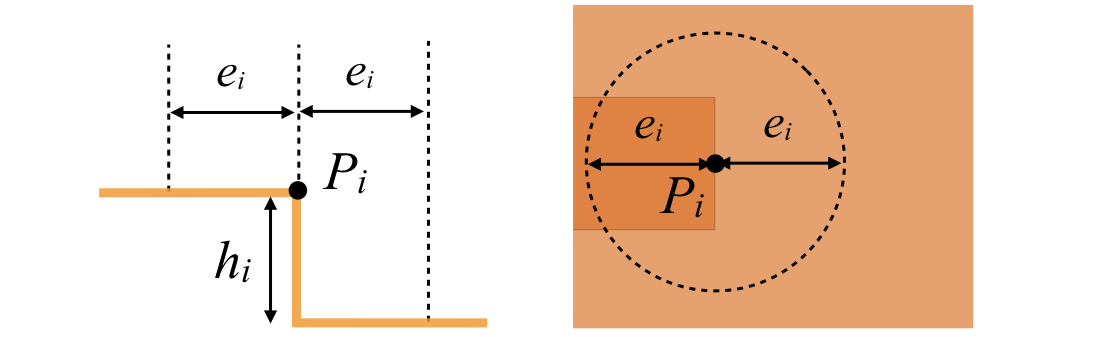
\includegraphics[width=6in]{./images/mehul12.png}
\caption{$C_G$ exclusion where the centre of gravity of the vehicle is prohibited from landing}
\label{f:mehul12}
\end{figure}

\noindent This allows an exclusion zone $e_i$ to be defined around each protrusion where the vehicle's $C_G$ cannot enter for landing, as shown in Fig~\ref{f:mehul12}. 

\begin{figure}[!ht]
\centering
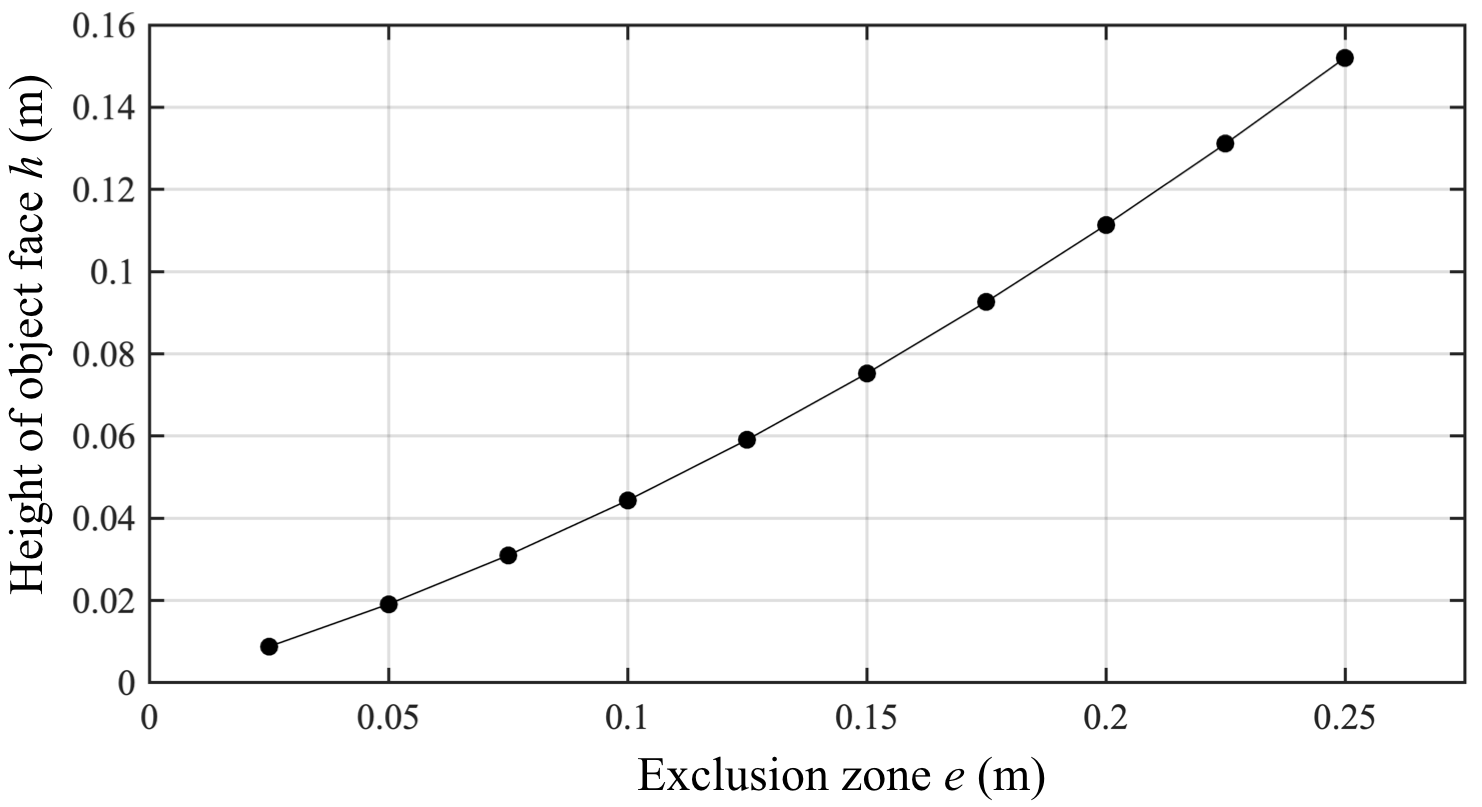
\includegraphics[width=5.5in]{./images/mehul13.png}
\caption{Exclusion zone for height of objects faces}
\label{f:mehul13}
\end{figure}

For the vehicle in Table.\ref{t:table2}, the maximum protrusion height is determined to be $h_c=0.15$\,m, where for protrusions higher than $h_c$, the $C_G$ exclusion zone is set to half the length of the vehicle along a given landing heading $\alpha$. This prevents the vehicle in this heading from making contact with the protrusion. For protrusions $h<h_c$, the $C_G$ exclusion zone calculated in steps of $5$ mm equivalent to the mapping resolution for the dimensions of the vehicle is seen in Fig~\ref{f:mehul13}, where protrusions $<5$ mm are not considered as protrusions since they cannot be distinguished from noise. The flowchart of the algorithm for landing area and exclusion zone detection is seen in Fig~\ref{f:mehul14}.\\
%However, since most vehicles are not circular in shape, the $C_G$ exclusion zone for these points can be calculated based on the geometry of the vehicle and the heading during landing $\alpha$. This will also reduce the size of the $C_G$ exclusion zone.  Using the conditions identified for safe landing, t
\begin{figure}[!ht]
\centering
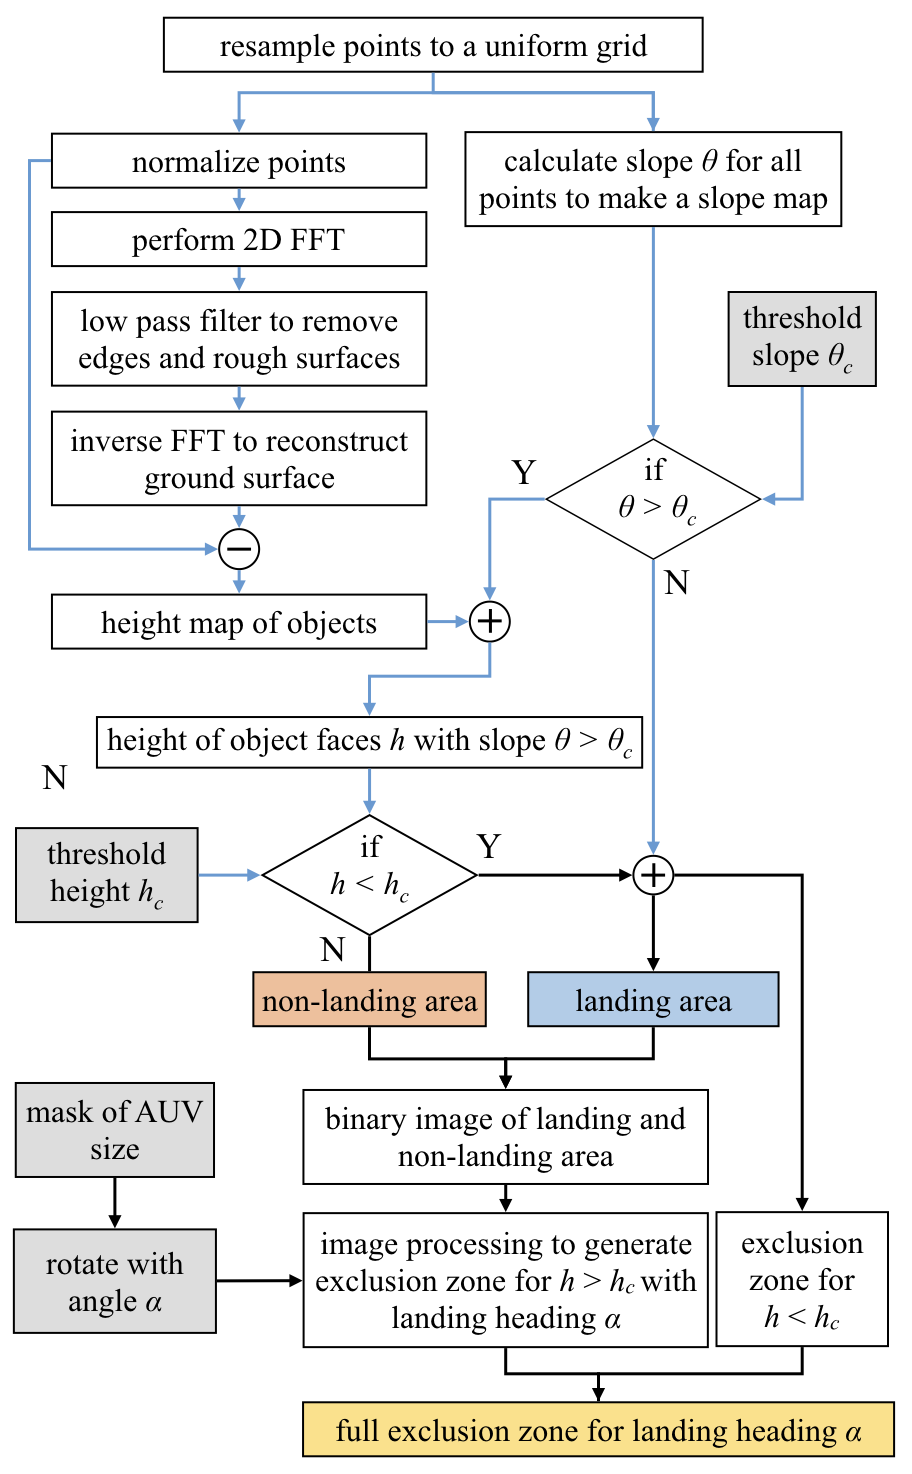
\includegraphics[width=4in]{./images/mehul14.png}
\caption{Flowchart for detection of landing area and generation of $C_G$ exclusion zone}
\label{f:mehul14}
\end{figure}

%In order to demonstrate the algorithm in Fig~\ref{f:mehul14}, a slope map is generated for the resampled point cloud. Two vectors are computed from three neighboring points making a triangle whose cross product is taken to find the normal vector. The angle of this normal vector to the horizontal is then calculated as the slope. 
%, where the slope is calculated for t is seen in 


In order to demonstrate the algorithm in Fig~\ref{f:mehul14}, data collected is analysed assuming the vehicle parameters given in Table.\ref{t:table2}. Fig.~\ref{f:slope_analysis}a shows the slope map generated for the three areas A,B and C. The slope threshold $\theta_c= 17.7^\circ$ is applied to generate the binary map Fig.~\ref{f:slope_analysis}b.

\begin{figure}[!ht]
\centering
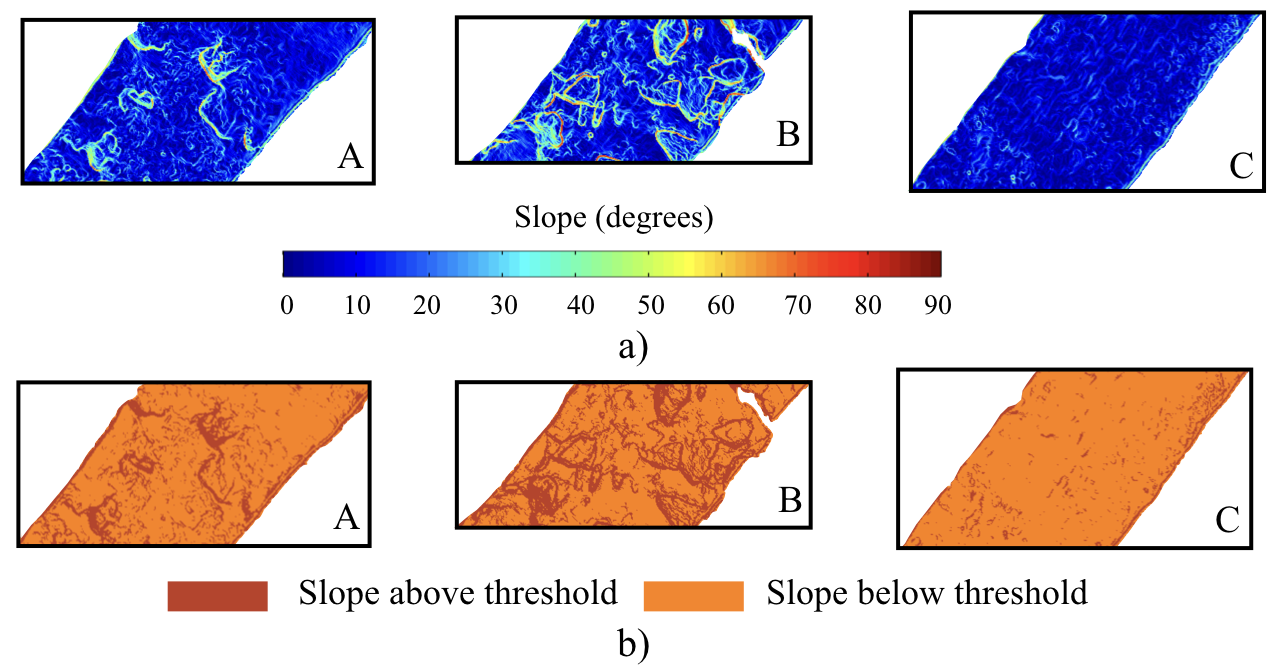
\includegraphics[width=6in]{./images/mehul15.png}
\caption{a) Slope calculated for areas A B and C. Area B shows objects having faces with higher slope than block C and A. Area C shows more smoother surface with less slope b) Slope threshold map for the three areas }
\label{f:slope_analysis}
\end{figure}

To analyse protrusions, two dimensional Fourier analysis is performed on the uniformly resampled bathymetry. The points in the area are zero filled on all sides to form a $N \times N$ matrix, where $N$ is the next power of $2$ more than the largest dimension of the area. The depth values of the points are normalized to remove the zero frequency component by subtracting the mean depth value and aligning the points with their Eigenvectors. A two dimensional $N$ point Fast Fourier Transform (FFT) is performed on the normalized values to convert them to the frequency domain. The frequency bins are $n \times f_s/N$, where $n = 1, 2, \dots, N/2$ and sampling frequency is $f_s = 1/g_{res}$. A low pass filter is applied where for a cut-off frequency $f_c$, filter order $n$ and frequency bins $f$

%The Frequency content of these profiles is analyzed for separating objects from the ground surface. Flat areas are dominated by low frequency components of the profiles while the high frequency components represent the sharp edges of objects and rough surfaces. Analysis is performed on in each area using a two dimensional Fast Fourier Transform (FFT). The points in the area are zero filled on all sides to form a $N \times N$ matrix, where $N$ is the next power of $2$ more than the largest dimension of the area. The depth values of the points are then normalized to remove the DC component by subtracting the mean depth value and rotated along their Eigenvectors. Two dimensional $N$ point FFT is performed on the normalized values to convert them to frequency domain values. The frequency bins are $n \times f_s/N$, where $n = 1, 2, \dots, N/2$ and $f_s = 1/g_{res}$ the sampling frequency. A low pass filter with a linear phase response with nearly even response in the pass band and a sharp cut-off is applied to the frequency domain values to suppress the high frequency components. For cut-off frequency $f_c$, filter order $n$ and frequency bins $f$, the equation of the filter used is:

\begin{equation}
\label{eq:eq8}
\centering
	h_{l}(f) = \frac{1}{\sqrt{1 + (\frac{f}{f_c})^{2n}}}.
\end{equation}

A 3rd order filter is used to provide suitable sharpness of damping with $3$ dB attenuation at the cut-off frequency. This was determined using the method described in ~\cite{Lyons1997} ~\cite{Kalogerakis2010} as $f_c = 2/\sigma$, where $\sigma$ is taken as the diagonal length of the vehicle's geometry as a multiple of the sampling resolution. The filter function is rotated around the zero frequency to form a $N\times N$ point filter and multiplied to the frequency domain values element by element. An inverse two dimensional FFT produces smooth surface representing the low frequency component. This is subtracted from the unfiltered surface to generate a map of protrusions, as seen in Fig.~\ref{f:mehul19}.

%represents the minimum size of an the seafloor  at the ed by a step function, the equivalent sync function in frequency domain has first zero crossings at $2/\sigma$ . The cut-off frequency is set as $f_c = 2/\sigma$ which indicates the frequency represented by the size of the object at the sampling resolution. $f_c = 5$ is used in this work. 



\begin{figure}[!ht]
\centering
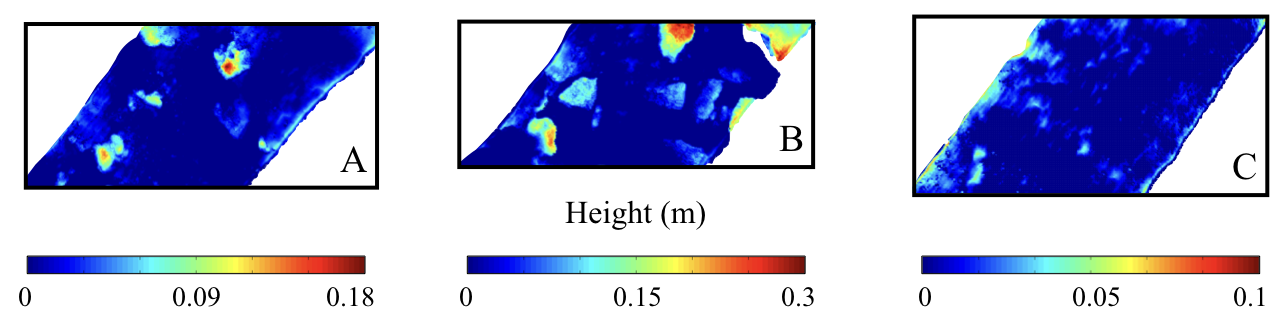
\includegraphics[width=6in]{./images/mehul19.png}
\caption{Height map for areas A B and C. Areas A and B show large objects on the seafloor compared to area C}
\label{f:mehul19}
\end{figure}

The height of protrusions $h$ is extracted in areas above the slope threshold $\theta > \theta_c$ from the height map of objects as in Fig.~\ref{f:mehul20_21}b. For $h < h_c$, the $C_G$ exclusion zone is generated using the relationship in Fig.~\ref{f:mehul13} giving the $C_G$ exclusion regions shown in Fig.~\ref{f:mehul20_21}c. For protrusions above the threshold $h > h_c$, the $C_G$ exclusion zone takes into account the landing heading $\alpha$ and the geometry of the vehicle so that the vehicle avoids making contact with the protrusion. To achieve this, binary image morphological operations are performed using a structural element with the vehicle's dimensions for a landing heading of $\alpha=55^\circ$ as shown in Fig.~\ref{f:mehul20_21}d. The two exclusion zone maps are superimposed in Fig.~\ref{f:mehul22}a to give the final exclusion zone map that is used for landing site identification.

%For this, location of all points having a certain height range are identified to form a binary image. Morphological dilation is then performed on this binary image using a circular structural element with radius equal to size of the exclusion zone for that height. <- I think this is pretty clear/not so important how you implemented it.

%For this, a rectangular structural with dimensions in pixels equal to the size of the vehicle is generated. The structural element is then rotated to the landing heading to generate a new structural element representing the rotated vehicle. <- same, the idea is valuable but the implementation is just simple.


% \begin{figure}[!ht]
% \centering
% 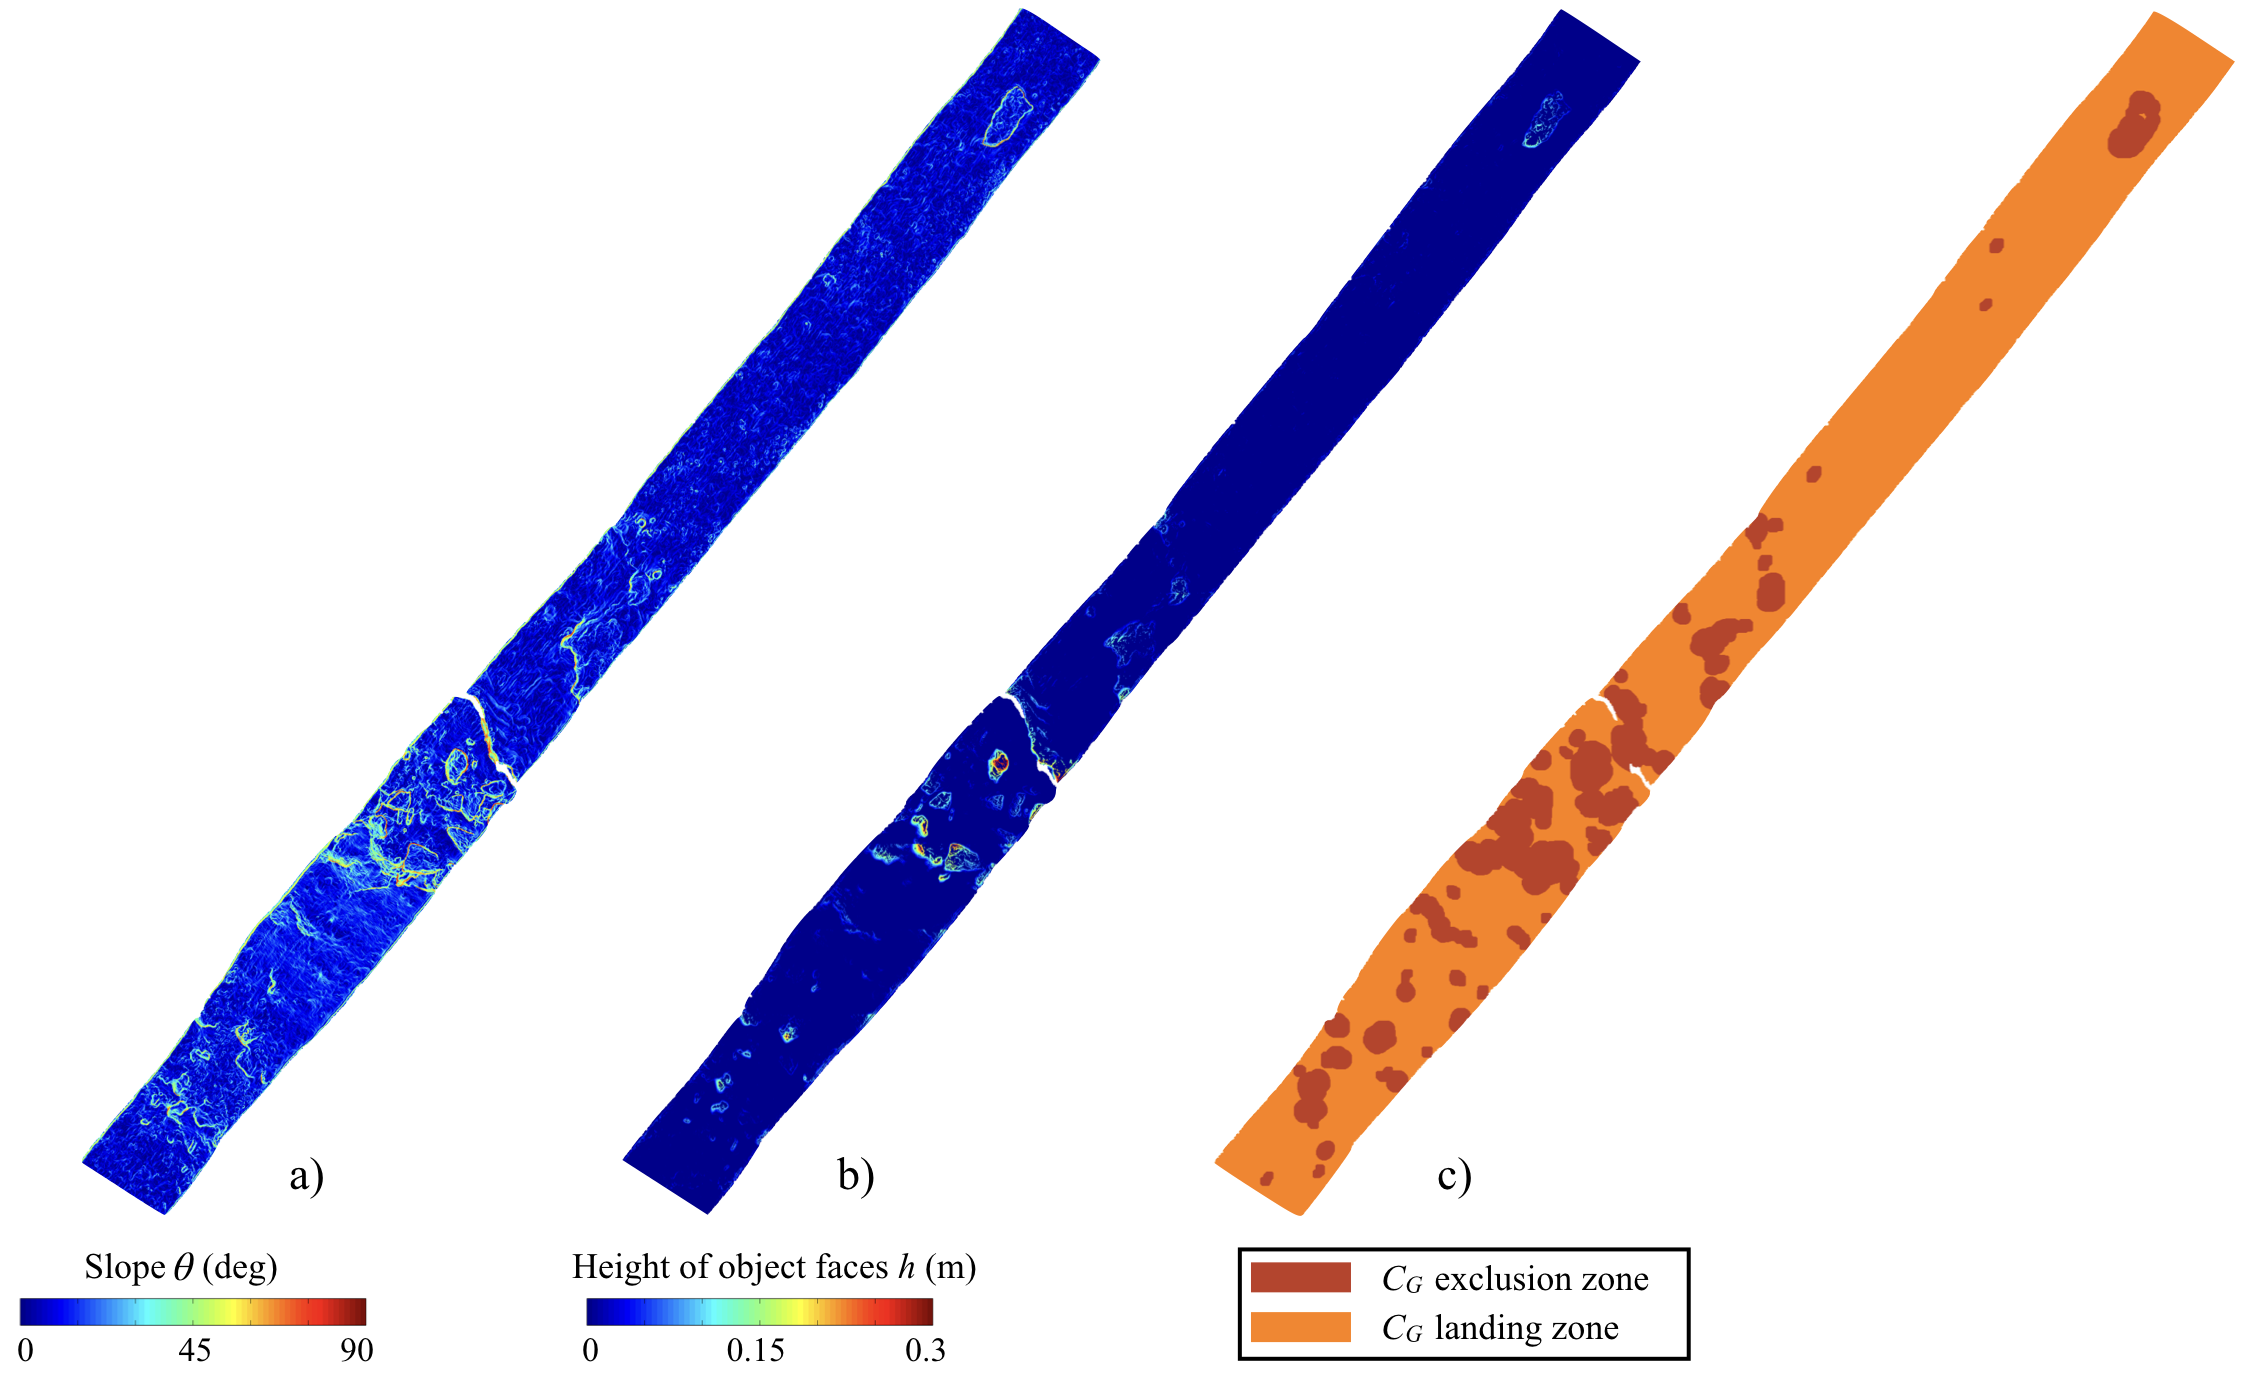
\includegraphics[width=5.5in]{./images/mehul20.png}
% \caption{a) Slope map of the mapped bathymetry b) Height of object faces $h$ for slope $\theta > \theta_c$ c) $C_G$ exclusion zone for object faces $h < h_c$}
% \label{f:mehul20}
% \end{figure}

% \begin{figure}[!ht]
% \centering
% 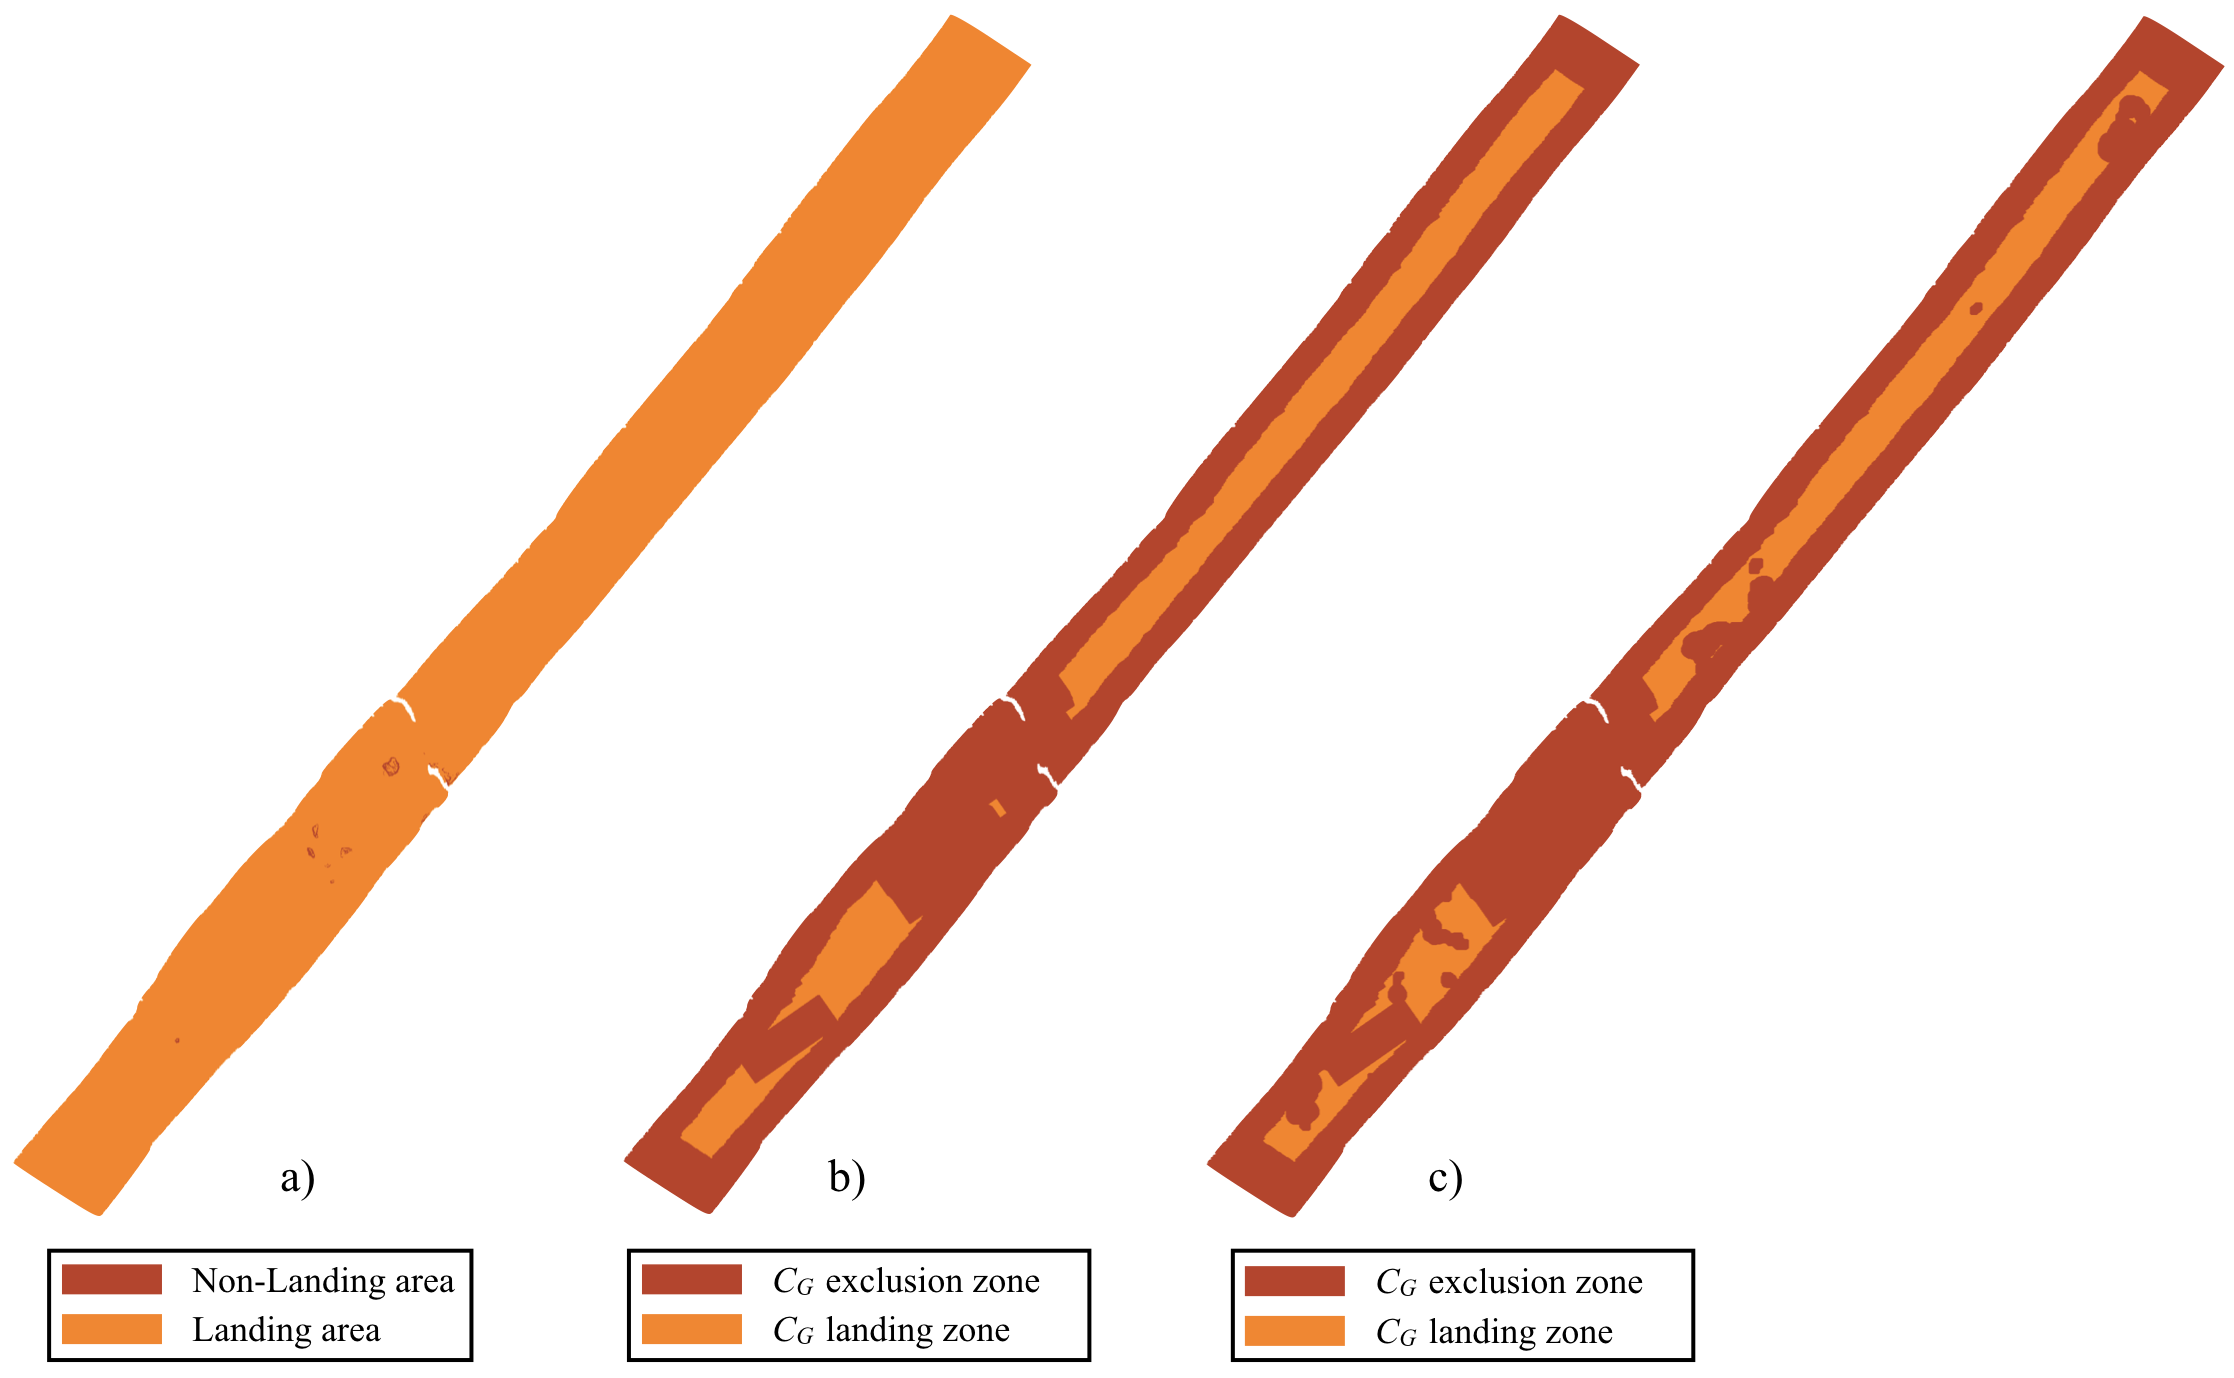
\includegraphics[width=5.5in]{./images/mehul21.png}
% \caption{a) Landing area for height threshold $h > h_c$ b)  $C_G$ Exclusion zone for landing area with $55^\circ$ landing heading  c) Full $C_G$ exclusion zone for protrusions $h < h_c$ and landing area with $55^\circ$ landing heading}
% \label{f:mehul21}
% \end{figure}

\begin{figure}[!ht]
\centering
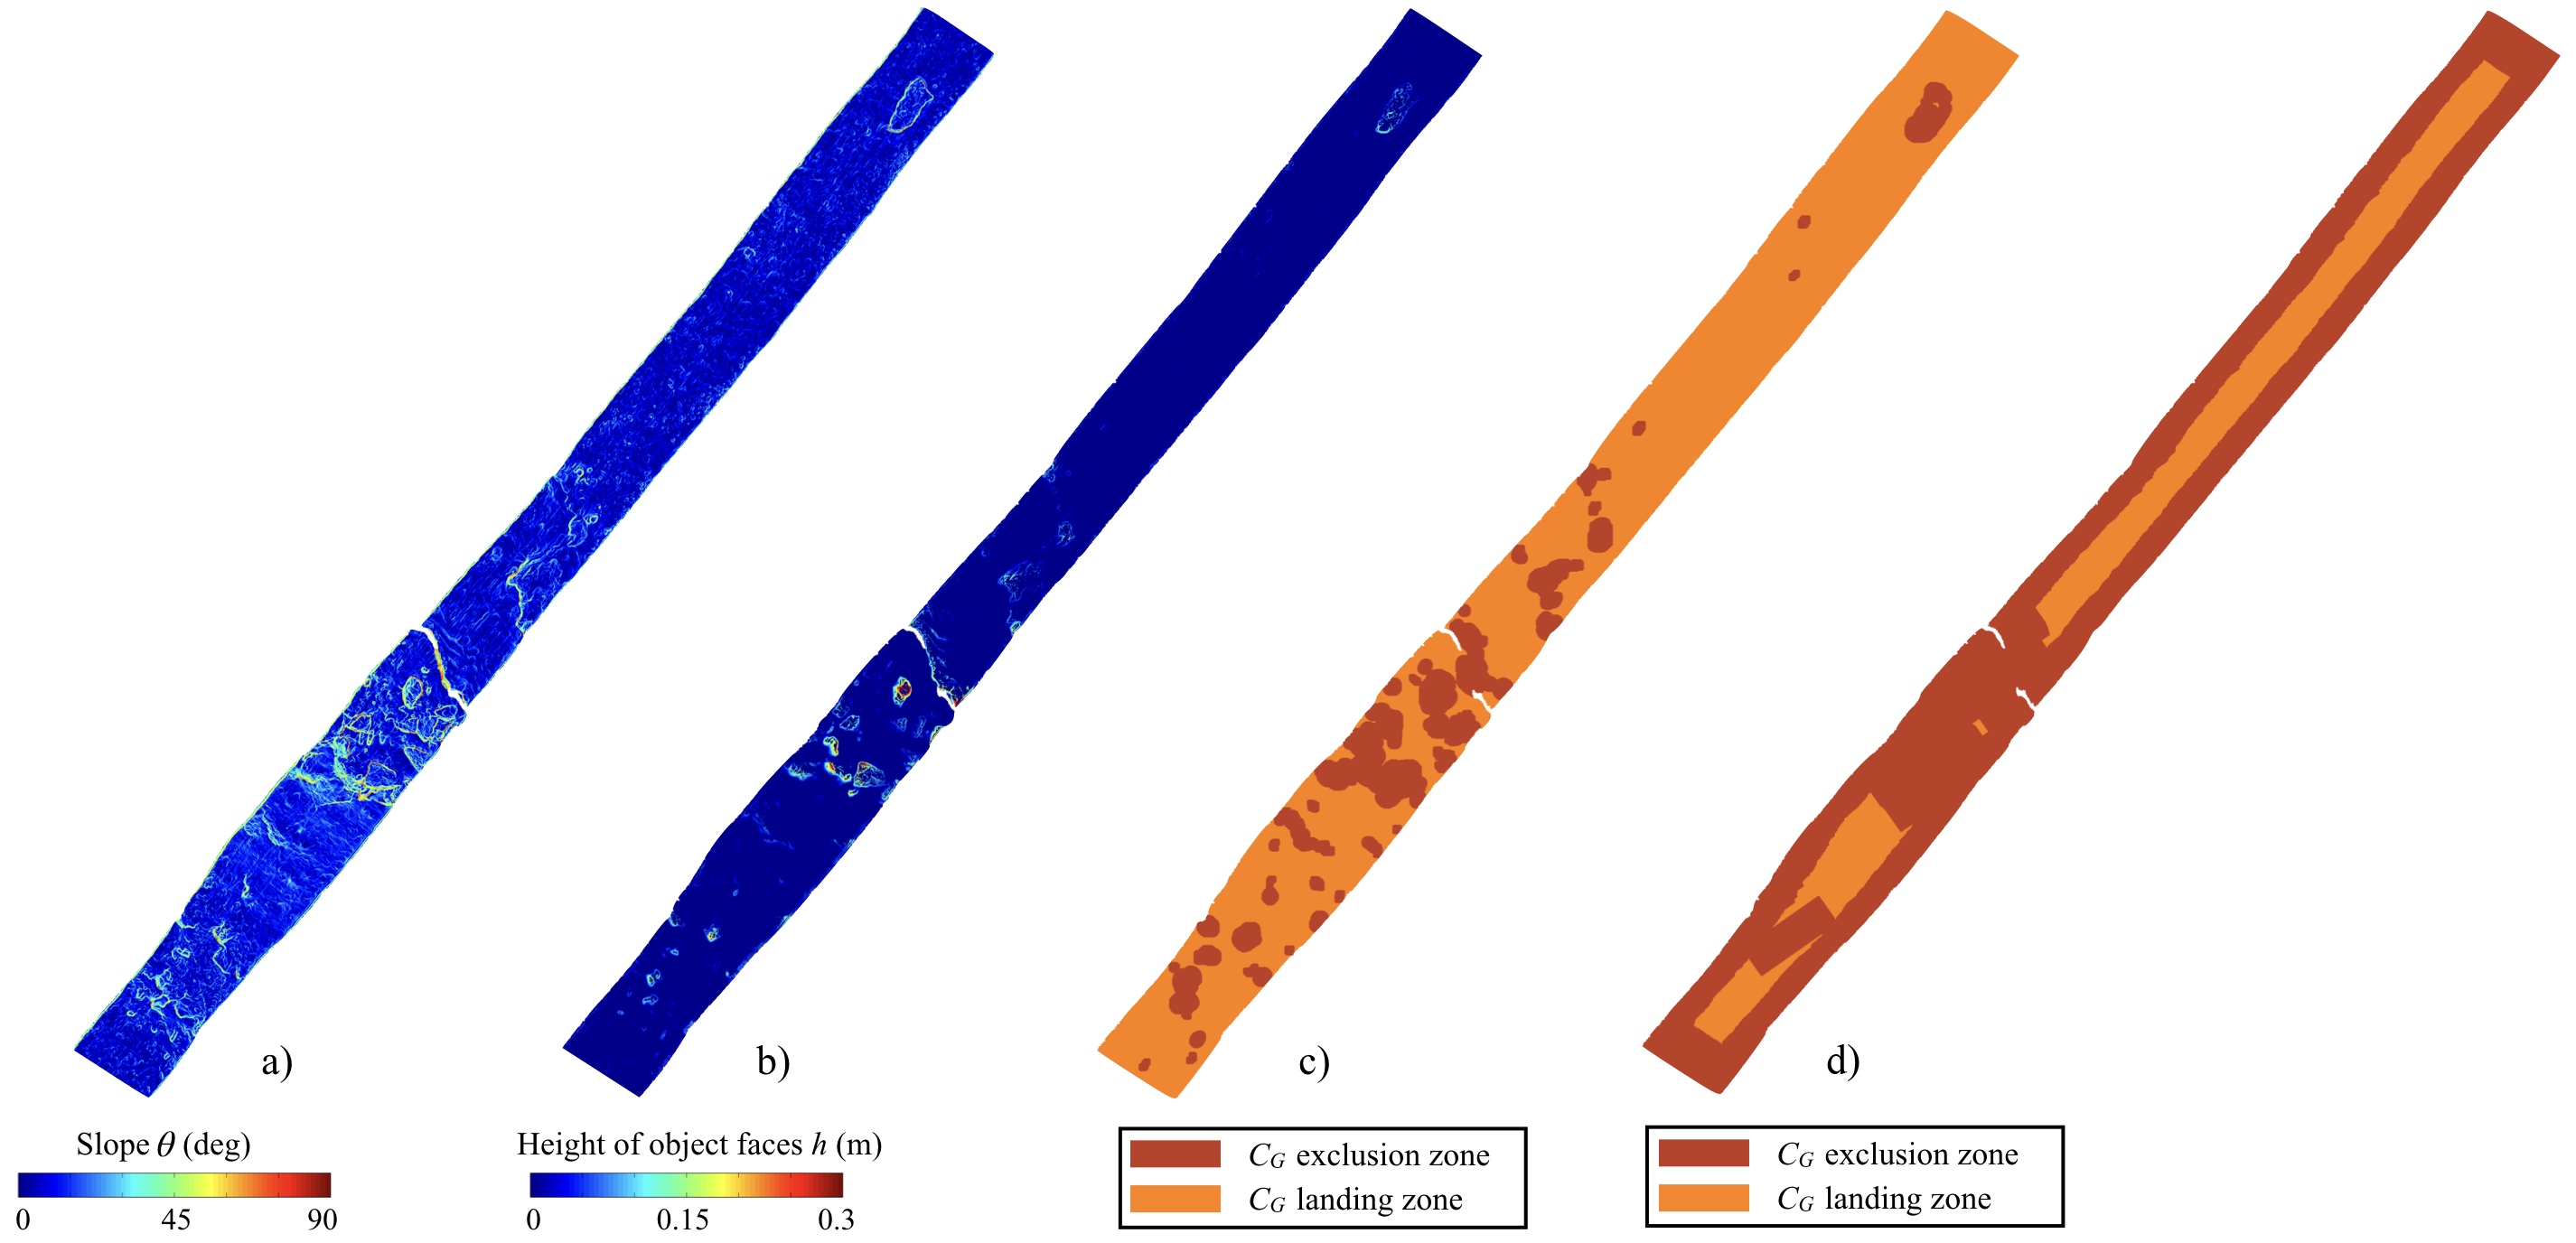
\includegraphics[width=6.5in]{./images/mehul20_21.png}
\caption{a) Slope map of the mapped bathymetry b) Height of object faces $h$ for slope $\theta > \theta_c$ c) $C_G$ exclusion zone for object faces $h < h_c$ d)  $C_G$ Exclusion zone for landing area with $55^\circ$ landing heading}
\label{f:mehul20_21}
\end{figure}
 
\subsection{Site identification}

Landing sites are identified by verifying the eight neighbor connectivity between pixels where the vehicle $C_G$ can land. A landing coordinate is calculated for each group of pixels where the vehicle can land furthest away from the group's boundary. This is achieved by determining the largest circle that can be inscribed within the group of pixels, where the centre of this circle is the landing coordinate. Groups where the radius of the largest inscribed circle is $<0.3$\,m are rejected considering AUV positioning errors when navigating back to each site. The remaining groups are labelled as candidate landing sites, where Fig~\ref{f:mehul22} shows the candidate sites identified for a vehicle heading of $55^\circ$.

\begin{figure}[!ht]
\centering
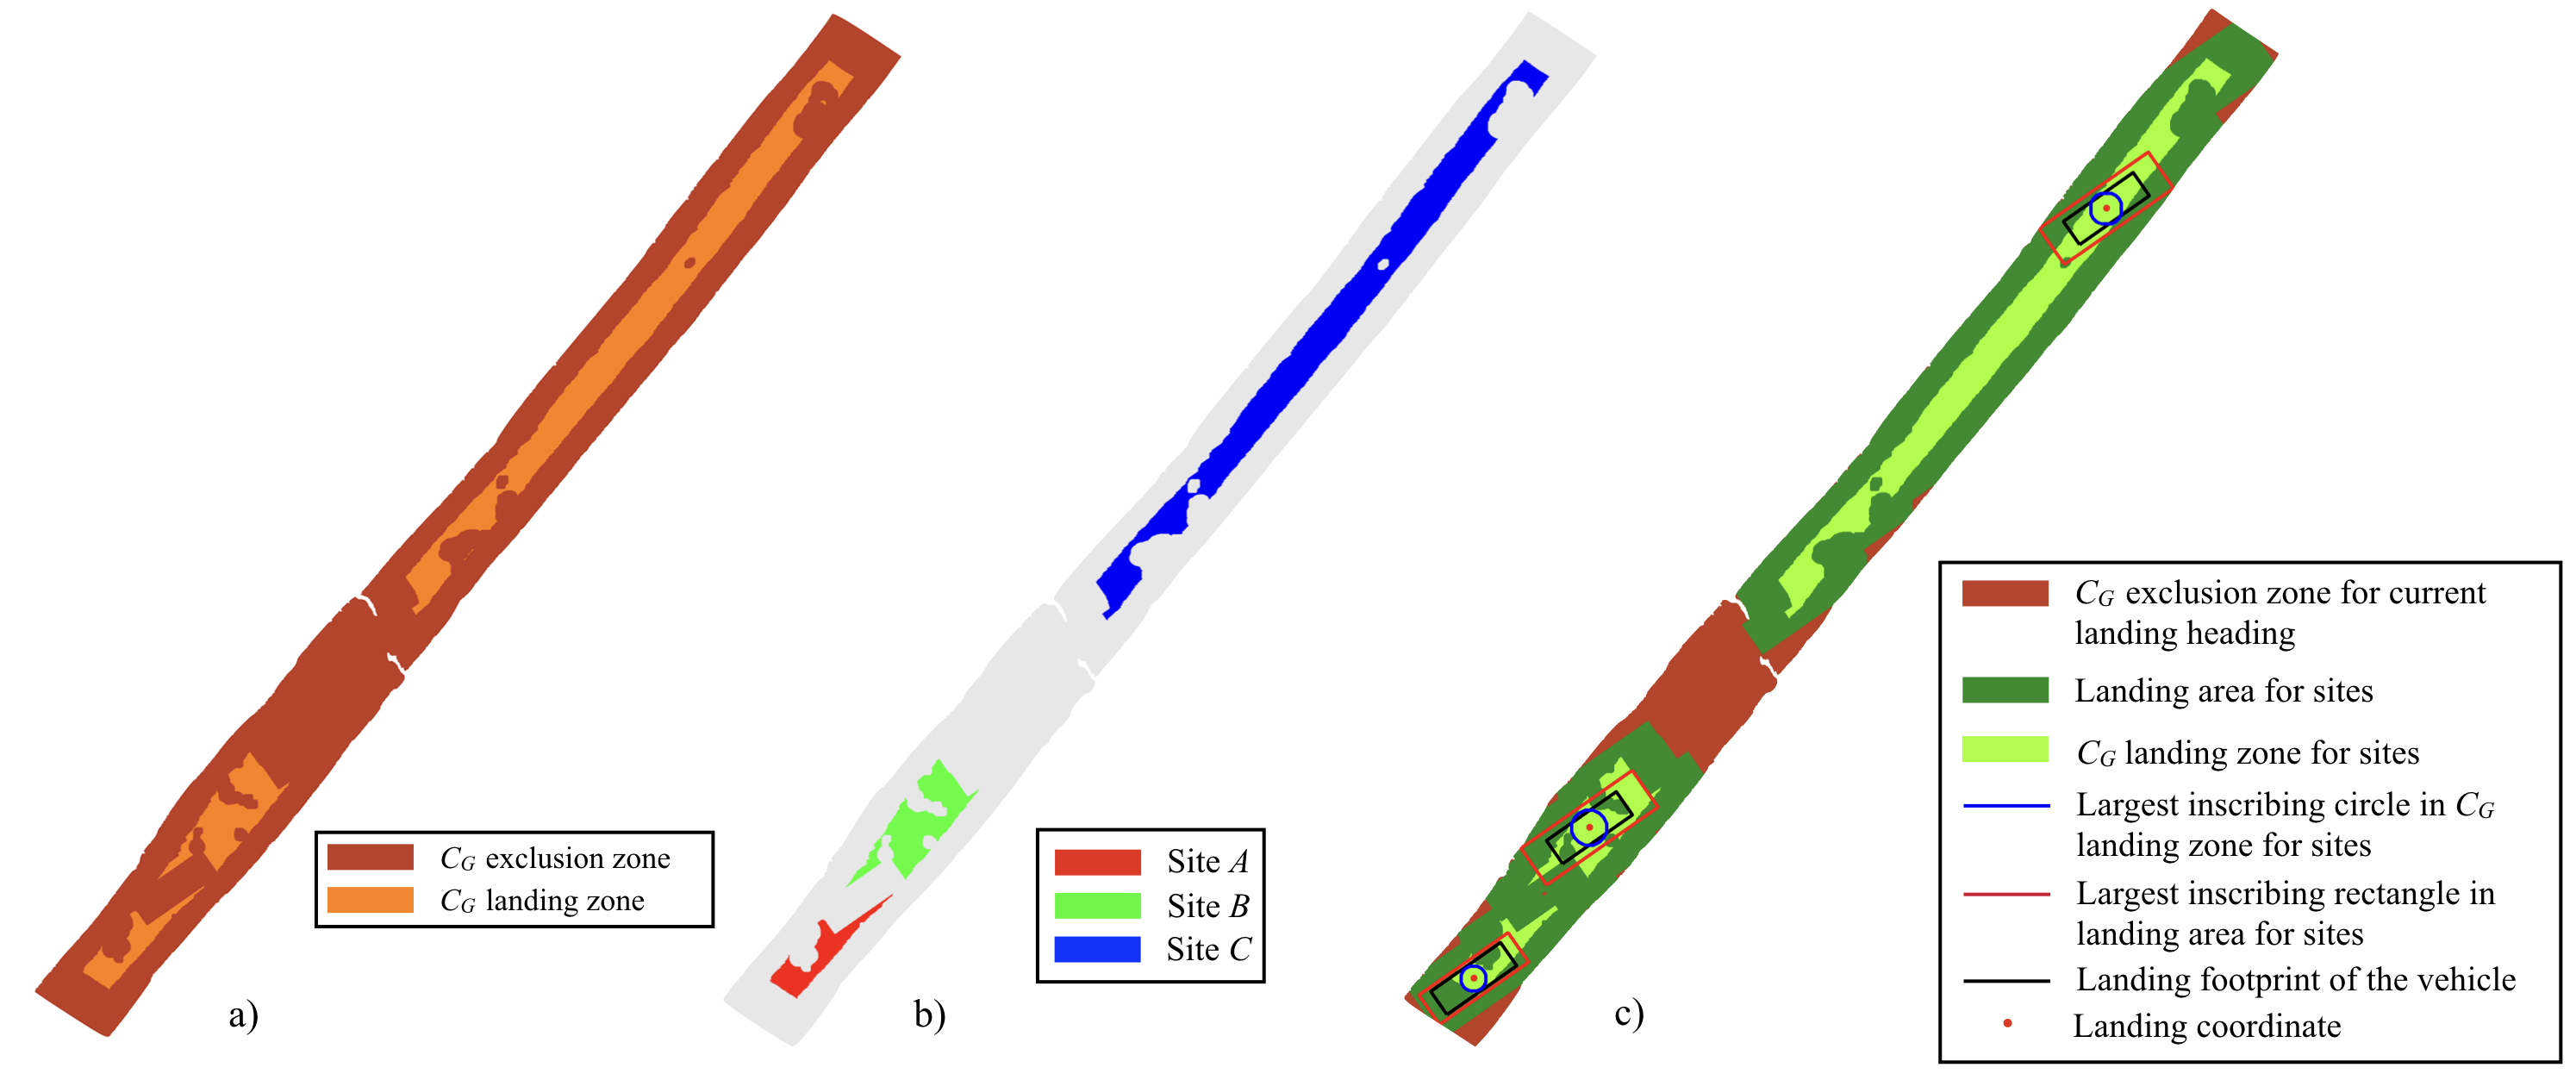
\includegraphics[width=6.5in]{./images/mehul22_BT.png}
\caption{a) Full $C_G$ exclusion zone for a $55^\circ$ landing heading, b) Landing sites identified for $55^\circ$ landing heading, and c) Landing point calculation }
\label{f:mehul22}
\end{figure}

Each candidate site is characterised by extracting the following seafloor properties from the within the footprint of the vehicle for each landing coordinate and heading, as illustrated in 	Fig~\ref{f:mehul22}c.

\begin{itemize}
  \item \textit{Slope $P_s$:} The mean landing slope $\overline{\theta}$ is calculated for the points in the landing footprint of the vehicle. The slope is normalized using the threshold slope $\theta_c$ to determine the slope cost as follows, 
\begin{equation}
\label{eq:eq9}
\centering
	P_s = \frac{\overline{\theta}}{\theta_c}.
\end{equation}
  \item \textit{Safety $P_f$:} Landing safety is determined by calculating the area of the largest rectangle with the same aspect ratio as the vehicle that can be inscribed in the landing site along the landing heading. The ratio of this area $A_r$ to the footprint of the vehicle $A_f$ is used to calculated the safety cost. Since beyond a certain ratio, having a larger area to land does not increase safety, the value of the cost $P_f$ is limited to between 0 and 1 as follows,
 \begin{equation}
 \label{eq:eq10}
    P_f = \frac{1}{4}\left( 5 - \frac{A_r}{A_f}\right) \hskip \mathrm{where} \hskip  0<P_f<1.
  \end{equation}
  \item \textit{Roughness $P_r$:} The mean deviation of height $h$ from the mean value $\overline{h}$ after subtracting the low frequency component is used to determine $R$ of the landing footprint. This is normalized by the maximum value of roughness possible, $R_{max}$, which is illustrated in Fig.~\ref{f:mehul22a}.
  \begin{equation}
  \label{eq:eq11}
	R = \frac{1}{n} \sum_{i=1}^{n}\left | h_i - \overline{h} \right |
  \end{equation} 
  \begin{equation}
  \label{eq:eq12}
	P_f = \frac{R}{R_{max}} 
  \end{equation}\\ 
\end{itemize}

\begin{figure}[!ht]
\centering
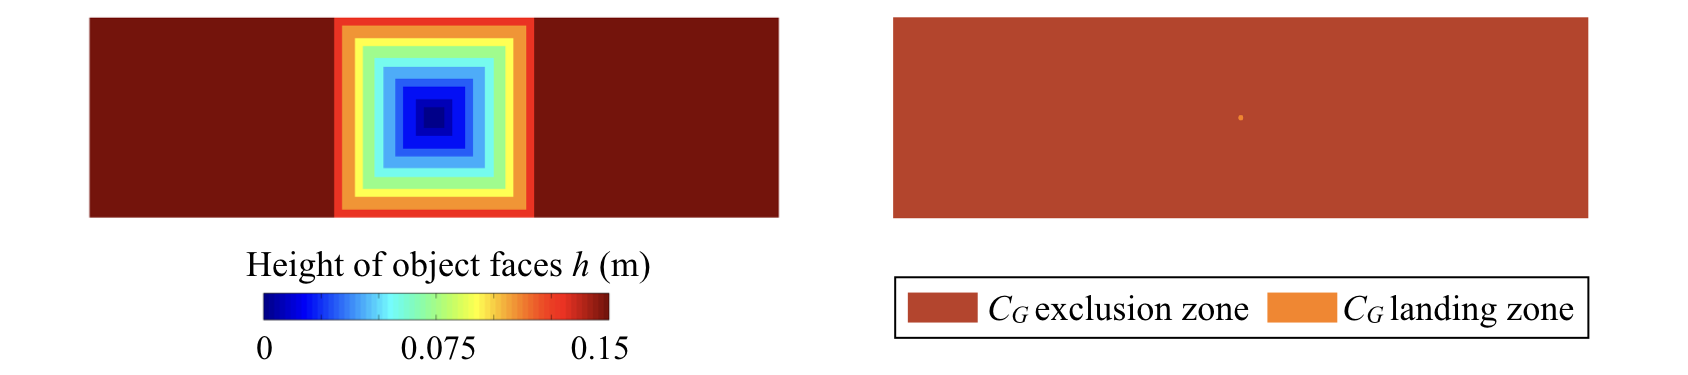
\includegraphics[width=6.5in]{./images/mehul22a.png}
\caption{Landing footprint of the vehicle showing the terrain corresponding to the largest value of roughness, $R_{max}$}
\label{f:mehul22a}
\end{figure}
 
\subsection{Site selection}
 
In order to select the most suitable landing site, the following cost function is defined based on the features of each candidate site,
 
 \begin{equation}
 \label{eq:eq13}
	C_s = \frac{1}{3}\left[P_s + P_f + P_r \right].
\end{equation} 

\noindent The candidate site with the lowest cost is selected as the most suitable landing site. The landing costs calculated for the three sites in Fig.\ref{f:mehul22}c are shown in Table~\ref{t:table4}, where in this case site C is the most suitable of the three candidates. 
   			
\begin{table}[!ht]
\centering
\caption{Landing site properties}
\begin{tabular}{  |p{2cm} p{2cm} p{2cm} p{2cm} p{2cm}| }
\hline
\textbf{Site} & \textbf{$P_s$} & \textbf{$P_f$} & \textbf{$P_r$} & \textbf{$C_s$}\\ \hline 
$A$ & $0.54$ & $0.85$ & $0.29$ & $0.56$ \\
$B$ & $0.67$ & $0.62$ & $0.32$ & $0.54$ \\
$C$ & $0.34$ & $0.65$ & $0.15$ & $0.38$ \\
\hline
\end{tabular}
\label{t:table4}
\end{table}

For each section of mapped bathymetry, the most suitable landing site is selected from candidates sites determined for multiple landing headings. These are calculated between $-90^\circ$ and $90^\circ$, where the costs for landing sites in the opposite direction are identical for a rectangular vehicle geometry. Costs are calculated in steps of $5^\circ$ to achieve a balance between resolution and computational cost. The landing costs calculated for all the landing candidates in the bathymetry shown in Fig.~\ref{sf:mehul4} are plotted in Fig.~\ref{f:mehul23}. The analysis shows that landing site $B$ for a landing heading of  $\alpha = 40^\circ$ has the lowest cost and is selected as the final landing site in this region of seafloor, with the properties of the site shown in Table ~\ref{t:table5}.


\begin{figure}[!ht]
\centering
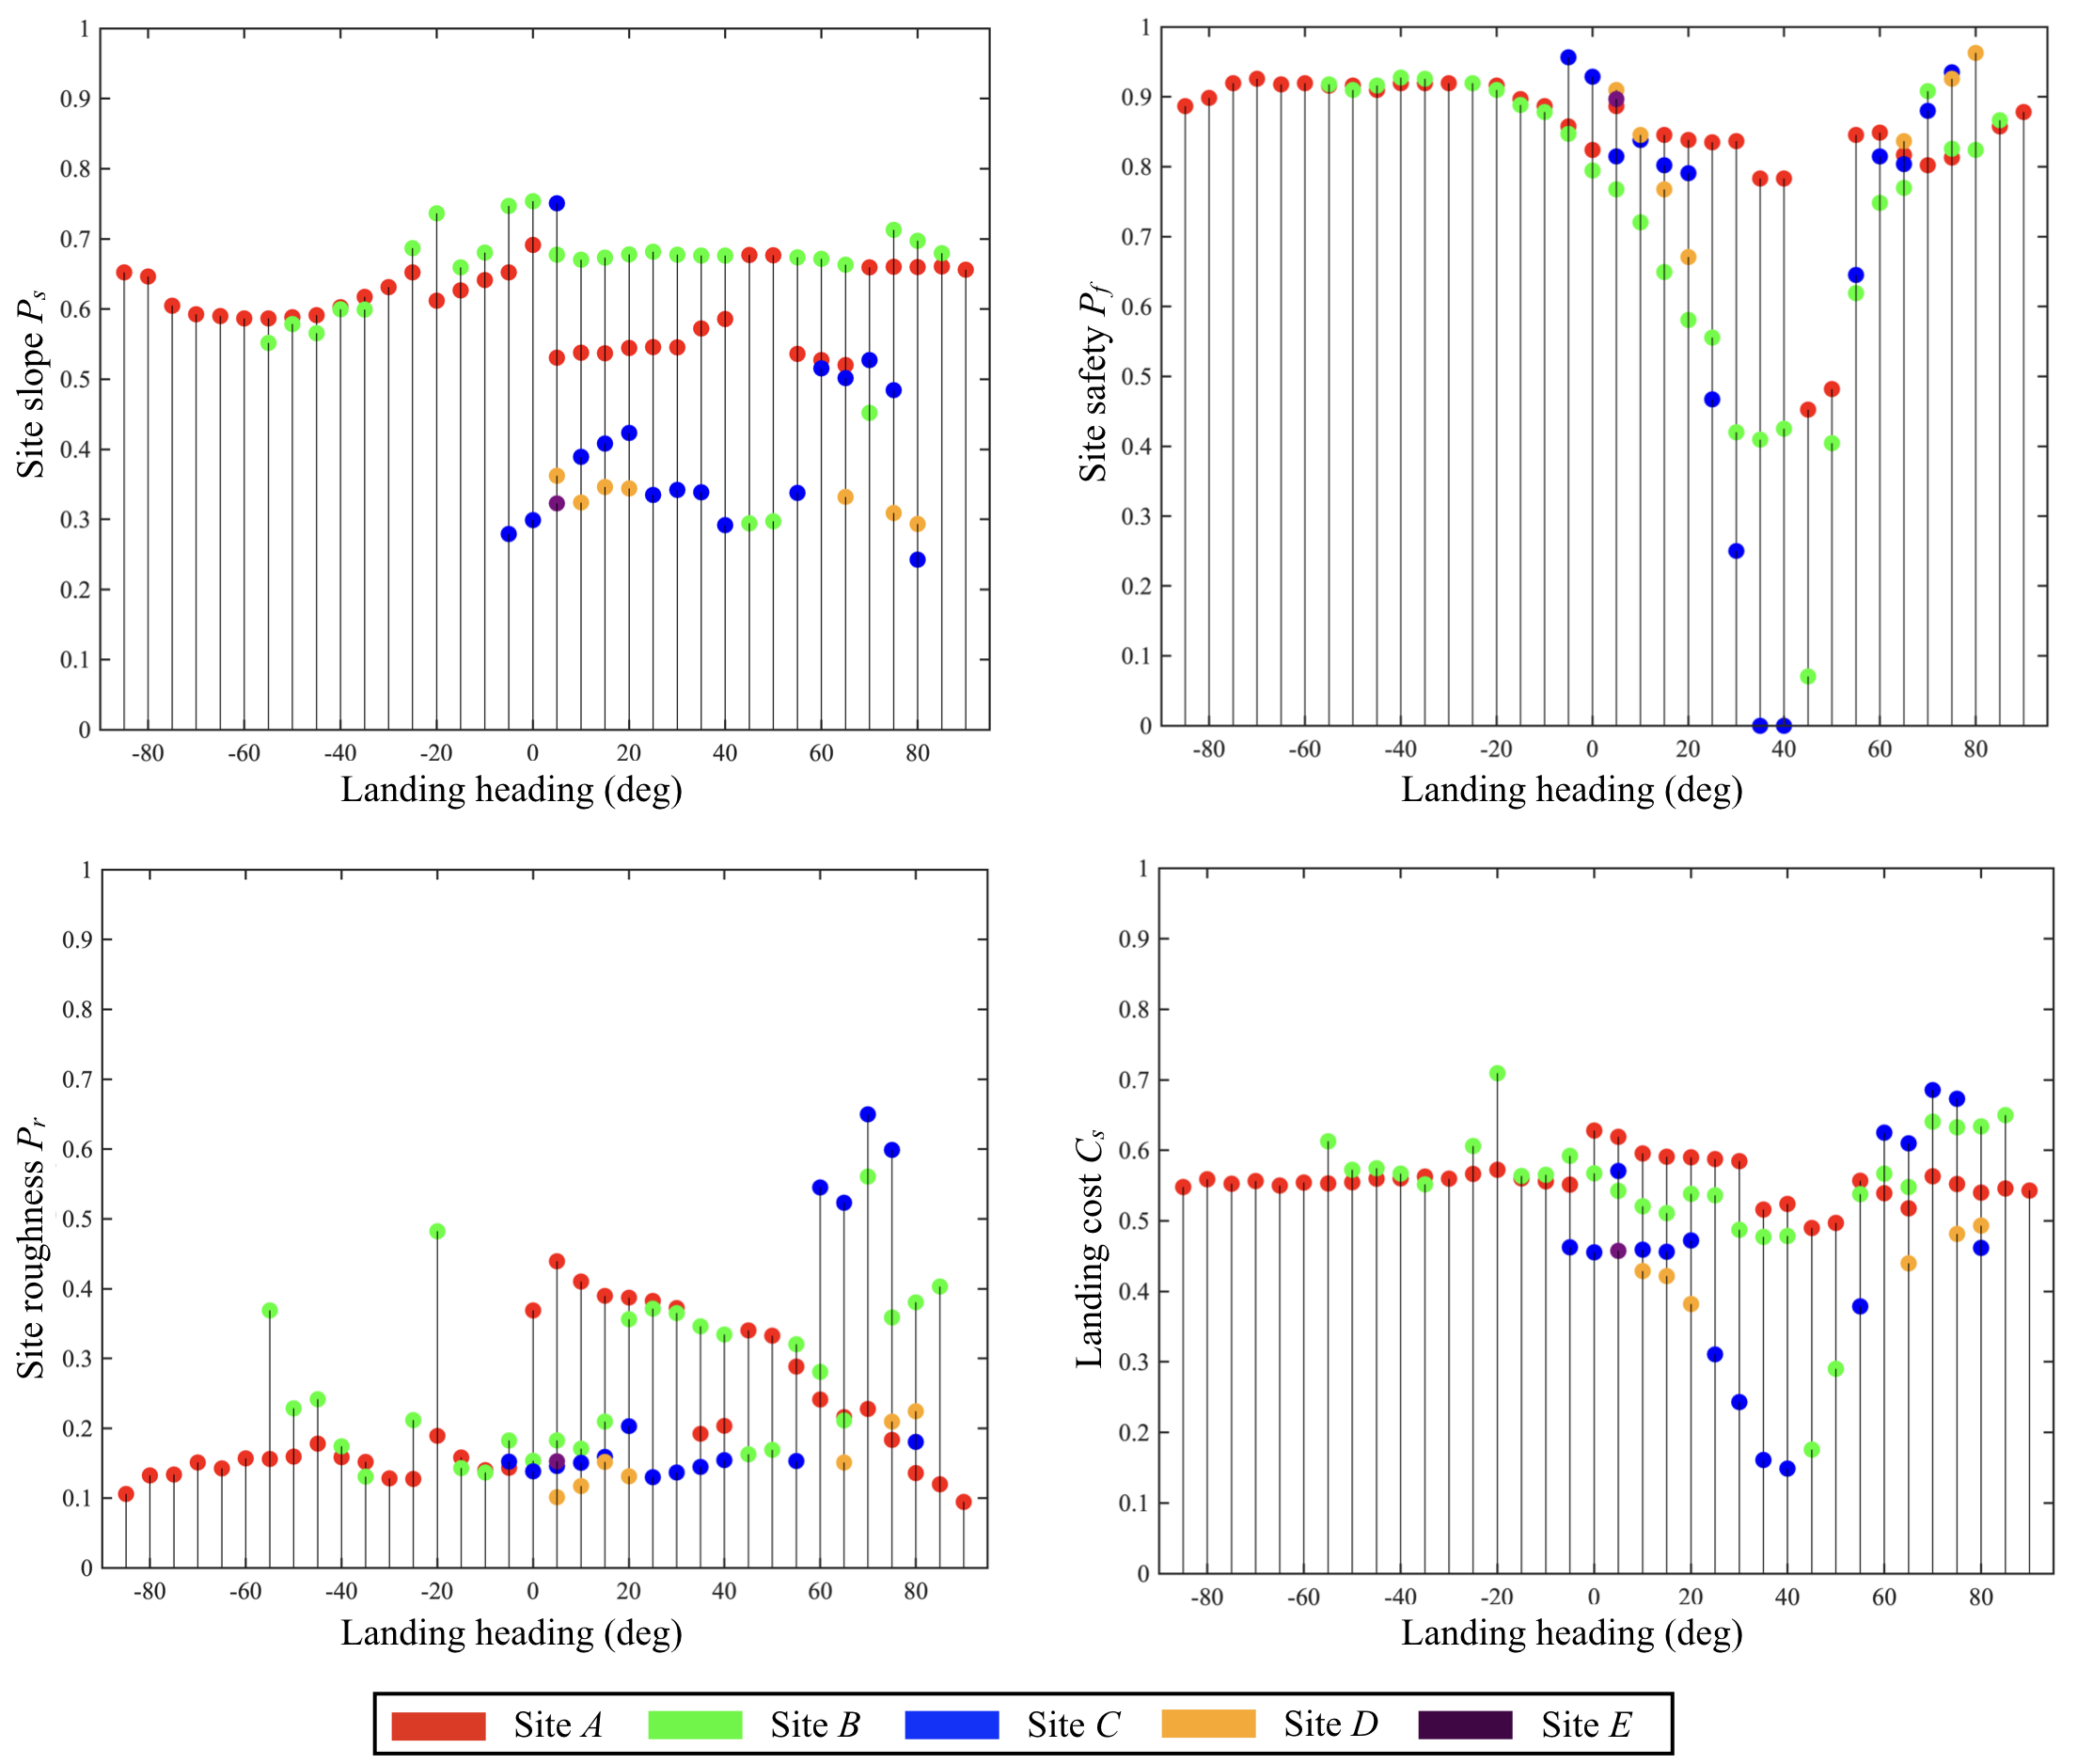
\includegraphics[width=\textwidth]{./images/mehul23.png}
\caption{Properties of the landing sites}
\label{f:mehul23}
\end{figure}


\begin{table}[!ht]
\centering
\caption{Properties for final landing site}
\begin{tabular}{  |p{6cm}  p{4cm}| }
\hline
\textbf{Property} & \textbf{Value}\\ \hline 
Landing heading & $40^\circ$ or $220^\circ$ \\
Mean depth & $1380$ m\\
$P_s$ & $0.29$\\
$P_f$ & $0.00$\\
$P_r$ & $0.16$\\
$C_s$ & $0.15$\\
\hline
\end{tabular}
\label{t:table5}
\end{table}
